\documentclass[a4paper, 11pt,reqno]{article}
\input{macro/package.tex}
\input{macro/environement}
% Header et footer

\pagestyle{fancy}
\fancyhead{}
\fancyfoot{}
\renewcommand{\headwidth}{\textwidth}
\renewcommand{\footrulewidth}{0.4pt}
\renewcommand{\headrulewidth}{0pt}
\renewcommand{\footruleskip}{5px}

\fancyfoot[R]{Olivier Glorieux}
%\fancyfoot[R]{Jules Glorieux}

\fancyfoot[C]{ Page \thepage }
\fancyfoot[L]{1BIOA - Lycée Chaptal}
%\fancyfoot[L]{MP*-Lycée Chaptal}
%\fancyfoot[L]{Famille Lapin}

\input{macro/newcommand.tex}
\geometry{hmargin=1.0cm, vmargin=2.5cm}


\newcommand{\type}{TD }
\excludecomment{correction}
%\newcommand{\type}{Correction TD }


\begin{document}
\title{\type 8 - Vocabulaires des Applications}

%-----------------------------------------------------------------------------------------------
\section*{Entraînements}

%------------------------------------------------
%-------------------------------------------------
\begin{exercice}  \;
	On consid\`ere l'application $f:\R\rightarrow\R$ d\'efinie par: $x  \mapsto  x^3-3x.$
	\begin{enumerate}
		\item
		      \'Etudier les variations de $f$.
		      %\item $f$ est-elle injective ?
		\item
		      D\'eterminer $f(\lbrack 1,2\rbrack)$, $f(\R)$, $f(\lbrack -1,+\infty\lbrack)$.
		      %\item 
		      %D\'eterminer $f^{-1}(\rbrack -2,+\infty\lbrack)$, $f^{-1}(\lbrace 0\rbrace)$.
	\end{enumerate}
\end{exercice}
\begin{correction} \;
	\begin{enumerate}
		\item \textbf{\'Etude de la fonction $\mathbf{f}$:}\\
		      \noindent $f$ est d\'efinie et d\'erivable sur $\R$ comme fonction polyn\^omiale.
		      $$\forall x\in \R,\ f^{\prime}(x)=3(x^2-1).$$
		      \begin{center}
			      \begin{tikzpicture}
				      \tkzTabInit{ $x$          /1,%
					      $f^{\prime}(x)$        /1,
					      $f$       /2}%
				      { $-\infty$ , $-1$ ,$1$, $+\infty$ }%
				      \tkzTabLine{,+,0,-,0,+}
				      \tkzTabVar{
					      -/ $- \infty$       /,%
					      +/ $2$       /,
					      -/$-2$        /,
					      +/$+\infty$    /,
				      }
			      \end{tikzpicture}
		      \end{center}
		      Les limites en l'infini s'obtiennent en utilisant le th\'eor\`{e}me du mon\^{o}me de plus haut degr\'e.
		      %\item \textbf{Montrons que $\mathbf{f}$ n'est pas injective de $\mathbf{\R}$ dans $\mathbf{\R}$:}\\
		      %\noindent 
		      %La fonction $f$ n'est pas injective de $\R$ sur $\R$.\\
		      %\noindent Par exemple, $f(-1)=2=f(2)$ et $-1\not= 2$.
		      %-----------------------
		\item \textbf{D\'eterminons $\mathbf{f(\lbrack 1,2\rbrack)}$, $\mathbf{f(\R)}$, $\mathbf{f(\lbrack -1,+\infty\lbrack)}$:}\\
		      \noindent
		      La recherche d'images directes se fait le plus souvent en utilisant le th\'eor\`{e}me de la bijection.
		      \begin{enumerate}
			      \item D\'eterminons $f(\lbrack 1,2\rbrack)$.\\
			            \noindent On peut par exemple utiliser le th\'eor\`eme de la bijection.
			            \begin{itemize}
				            \item[$\bullet$] $f$ est continue sur $\lbrack 1,2\rbrack$.
				            \item[$\bullet$]  $f$ est strictement croissante sur $\lbrack 1,2\rbrack$.
				            \item[$\bullet$] $f(1)=-2$ et $f(2)=2$.
			            \end{itemize}
			            Ainsi, par le th\'eor\`eme de la bijection, $f$ r\'ealise une bijection de $\lbrack 1,2\rbrack$ sur $\lbrack -2,2\rbrack$ et donc
			            $$\fbox{$f(\lbrack 1,2\rbrack)=\lbrack -2,2\rbrack.$}$$
			      \item
			            Il faut ici appliquer le th\'eor\`eme de la bijection sur chaque intervalle o\`u $f$ est strictement monotone, \`a savoir sur les intervalles $\rbrack -\infty, -1\rbrack$, $\lbrack -1,1\rbrack$ et $\lbrack 1,+\infty\lbrack$. On montre ainsi que \fbox{$f(\R)=\R$} et en particulier cela nous donne que la fonction $f$ est surjective de $\R$ sur $\R$.
			      \item
			            L\`a encore, en appliquant le th\'eor\`eme de la bijection sur les deux intervalles suivants $\lbrack -1,1\rbrack$ et $\lbrack 1,+\infty\lbrack$ o\`u la fonction $f$ est strictement monotone, on obtient \fbox{$f(\lbrack -1,+\infty\lbrack)=\lbrack -2,+\infty\lbrack$.}
		      \end{enumerate}
		      %--------------------------------
		      %\item \textbf{D\'eterminons $\mathbf{f^{-1}(\rbrack -2,+\infty\lbrack)}$ et $\mathbf{f^{-1}(\lbrace 0\rbrace)}$:}\\
		      %\noindent La recherche d'images r\'eciproques se fait le plus souvent en r\'esolvant une \'equation ou une in\'equation.
		      %\begin{enumerate}
		      %\item Par d\'efinition de l'image r\'eciproque d'une application, on a:\\
		      %\noindent $x\in f^{-1}( \rbrack -2,+\infty\lbrack)\Leftrightarrow f(x)>-2\Leftrightarrow x^3-3x>-2\Leftrightarrow x^3-3x+2>0\Leftrightarrow (x-1)(x^2+x-2)>0$. Un tableau de signe donne alors que \fbox{$f^{-1}( \rbrack -2,+\infty\lbrack)= \rbrack -2,+\infty\lbrack$.}
		      %\item Par d\'efinition de l'image r\'eciproque d'une application, on a:\\
		      %\noindent $x\in f^{-1}( \lbrace0 \rbrace)\Leftrightarrow f(x)=0\Leftrightarrow x^3-3x=0\Leftrightarrow x(x^2-3)=0.$
		      %Ainsi on obtient que \fbox{$f^{-1}( \lbrace 0 \rbrace)=\lbrace -\sqrt{3},0,\sqrt{3}\rbrace$.}
		      %\end{enumerate}
	\end{enumerate}
\end{correction}









%-------------------------------------------------







%-----------------------------------------------
\begin{exercice}  \;
	Soit $f$ l'application de $\bC$ dans $\R$ qui, \`{a} tout complexe associe son module. %Dans chacun des cas suivants, d\'eterminer l'image directe de $A$ et l'image r\'eciproque de $B$ par $f$.
	\\
	%\begin{enumerate}
	\begin{minipage}[t]{0.55\textwidth}
		\item Calculer l'image directe par $f$ de :
		\begin{enumerate}
			\item $A=\left\lbrace z\in\bC,\ \exists x\in\R,\ z=x+2i\right\rbrace$
			\item $A=\left\lbrace z\in\bC,\ \exists x\in\R,\ z=(1+\cos{(x)})+i\sin{(x)}\right\rbrace$.
		\end{enumerate}
	\end{minipage}
	%\begin{minipage}[t]{0.35\textwidth}
	%\item Calculer l'image r\'eciproque de :
	%\begin{enumerate}
	%\item $B=\lbrack -1,1\rbrack$.
	%\item $B=\R^{\star}_+$.
	%\end{enumerate}
	%\end{minipage} 
	%\end{enumerate}
\end{exercice}
\begin{correction} \;
	\begin{enumerate}
		\item
		      \begin{enumerate}
			      \item \textbf{Calcul de $\mathbf{f(A)}$ avec $\mathbf{A=\left\lbrace z\in\bC,\ \exists x\in\R,\ z=x+2i\right\rbrace}$:}\\
			            \noindent  Par d\'efinition d'une image directe par une application, on sait que
			            $f(A)=\lbrace y\in\R^+,\ \exists z\in A,\ y=f(z)\rbrace$. Et par d\'efinition de l'application $f$, on obtient que:
			            $f(A)=\lbrace y\in\R^+,\ \exists z\in A,\ y=|z|\rbrace$. Puis par d\'efinition de l'ensemble $A$, on a:
			            $f(A)=\lbrace y\in\R^+,\ \exists x\in \R,\ y=|x+2i| \rbrace=\lbrace y\in\R^+,\ \exists x\in \R,\ y=\sqrt{x^2+4} \rbrace=\lbrace \sqrt{x^2+4},\ x\in\R\rbrace=\lbrack 2,+\infty\lbrack$. Il suffit en effet d'\'etudier la fonction $g: x\mapsto \sqrt{x^2+4}$ pour obtenir que $g(\R)=\lbrack 2,+\infty\lbrack$.
			            %--
			      \item \textbf{Calcul de $\mathbf{f(A)}$ avec $\mathbf{A=\left\lbrace z\in\bC,\ \exists x\in\R,\ z=(1+\cos{(x)})+i\sin{(x)}   \right\rbrace}$:}\\
			            \noindent
			            Par d\'efinition d'une image directe par une application, on sait que
			            $f(A)=\lbrace y\in\R^+,\ \exists z\in A,\ y=f(z)\rbrace$. Et par d\'efinition de l'application $f$, on obtient que:
			            $f(A)=\lbrace y\in\R^+,\ \exists z\in A,\ y=|z|\rbrace$. Puis par d\'efinition de l'ensemble $A$, on a:
			            $$\begin{array}{lll}
					            f(A) & = & \lbrace y\in\R^+,\ \exists x\in \R,\ y=|1+\cos{x}+i\sin{x}| \rbrace=\left\lbrace y\in\R^+,\ \exists x\in \R,\
					            y=\sqrt{(1+\cos{x})^2+\sin^2{x}} \right\rbrace\vsec                                                                      \\
					                 & = & \left\lbrace y\in\R^+,\ \exists x\in \R,\
					            y=\sqrt{4\cos^2{\left( \ddp\frac{x}{2}\right)}} \right\rbrace=\left\lbrace y\in\R^+,\ \exists x\in \R,\
					            y=2\left| \cos{\left( \ddp\frac{x}{2}\right)} \right| \right\rbrace=\lbrack 0,2\rbrack
				            \end{array}$$ car $\left| \cos{\left( \ddp\frac{x}{2}\right)} \right| $ prend toutes les valeurs possibles entre 0 et 1 car \fbox{$f(A)=\lbrack 0,2\rbrack$.}
		      \end{enumerate}
		      %------
		\item
		      \begin{enumerate}
			      \item \textbf{Calcul de $\mathbf{f^{-1}(B)}$ avec $\mathbf{B= \lbrack -1,1\rbrack}$:}\\
			            \noindent  Par d\'efinition de l'image r\'eciproque d'une application, on cherche $z \in \bC$ tel que :
			            $$f(z) \in B \; \Leftrightarrow \; |z| \in [-1,1] \; \Leftrightarrow \;  -1\leq |z| \leq 1.$$
			            La premi\`ere in\'egalit\'e \'etant toujours vraie, on a $f^{-1}(B)= \lbrace z\in\bC,\  |z| \leq 1 \rbrace$ : l'ensemble \fbox{$f^{-1}(B)$ est donc le disque unit\'e ferm\'e de $\R^2$.}
			            %-----
			      \item \textbf{Calcul de $\mathbf{f^{-1}(B)}$ avec $\mathbf{B=\R^\star_+}$:}\\
			            \noindent  Par d\'efinition de l'image r\'eciproque d'une application, on cherche $z \in \bC$ tel que $|z| > 0$, ce qui correspond aux complexes non nuls. Ainsi \fbox{$f^{-1}(B) = \bC^\star$}.
		      \end{enumerate}
	\end{enumerate}
\end{correction}
%-----------------------------------------------



%---------------------------------------------------
%-------------------------------------------------
%-------------------------------------------------
%--------------------------------------------------
%----------------------------------------------------------------------------------------------
%-----------------------------------------------------------------------------------------------


%XXXXXX A REVOIR   

%------------------------------------------------------------------
\begin{exercice}  \;
	\'Etudier l'injectivit\'e, la surjectivit\'e et la bijectivit\'e des applications suivantes. Lorsqu'elles sont bijectives, d\'eterminer les applications r\'eciproques.
	\begin{enumerate}
		\begin{minipage}[t]{0.3\textwidth}
			\item $f:\left|\begin{array}{ccc} \R^+&\rightarrow& \R\vsec\\ x & \mapsto & \sqrt{x}\end{array}\right.$
			\item $f:\left|\begin{array}{ccc} \R^+&\rightarrow& \R^+\vsec\\ x & \mapsto & \sqrt{x}\end{array}\right.$
			\item $f:\left|\begin{array}{ccc} \R^+&\rightarrow& \R^+\vsec\\ x & \mapsto & x+1\end{array}\right.$
			\item $f:\left|\begin{array}{ccc} \R&\rightarrow& \R\vsec\\ x & \mapsto & x+1\end{array}\right.$
			\item $f:\left|\begin{array}{ccc} \R&\rightarrow& \R\vsec\\ x & \mapsto & |x|\end{array}\right.$
			\item $f:\left|\begin{array}{ccc} \R^+&\rightarrow& \R\vsec\\ x & \mapsto & |x|\end{array}\right.$
		\end{minipage}
		\begin{minipage}[t]{0.3\textwidth}
			\item $f:\left|\begin{array}{ccc} \lbrack -1,1\rbrack &\rightarrow& \lbrack 0,1\rbrack\vsec\\ x & \mapsto & |x|\end{array}\right.$
			\item $f:\left|\begin{array}{ccc} \R&\rightarrow& \R\vsec\\ x & \mapsto & x^3\end{array}\right.$
			\item $f:\left|\begin{array}{ccc} \R&\rightarrow& \R\vsec\\ x & \mapsto & x^4\end{array}\right.$
			%\item $f:\left|\begin{array}{ccc} \R^+&\rightarrow& \R\vsec\\ x & \mapsto & x^4\end{array}\right.$
			\item $f:\left|\begin{array}{ccc} \R^+&\rightarrow& \R^+\vsec\\ x & \mapsto & x^4\end{array}\right.$
			\item $f:\left|\begin{array}{ccc} \R&\rightarrow& \R\vsec\\ x & \mapsto & x^5\end{array}\right.$
			\item $f:\left|\begin{array}{ccc} \R&\rightarrow& \R\vsec\\ x & \mapsto & x^n\end{array}\right.$, $n\in\N^{\star}$
		\end{minipage}
		\begin{minipage}[t]{0.36\textwidth}
			\item $f:\left|\begin{array}{ccc} \R&\rightarrow& \rbrack 1,+\infty\lbrack \vsec\\ x & \mapsto & e^{-x}+1\end{array}\right.$
			\item $f:\left|\begin{array}{ccc} \rbrack -1,+\infty\lbrack&\rightarrow& \R \vsec\\ x & \mapsto & \ln{(1+x)}\end{array}\right.$
			\item $f:\left|\begin{array}{ccc} \R&\rightarrow& \rbrack -4,+\infty\lbrack \vsec\\ x & \mapsto & 2^x-4\end{array}\right.$
			%\item $f:\left|\begin{array}{ccc} \left\rbrack \ddp\frac{1}{3},+\infty\right\lbrack&\rightarrow& \R \vsec\\ x & \mapsto & \ln{(3x-1)}+5   \end{array}\right.$
			\item $f:\left|\begin{array}{ccc} \R&\rightarrow& \lbrack -\sqrt{2},\sqrt{2}\rbrack \vsec\\ x & \mapsto & \cos{(x)}+\sin{(x)}\end{array}\right.$
			\item $f:\left|\begin{array}{ccc} \Z&\rightarrow& \Z \vsec\\ n & \mapsto & 2n+1\end{array}\right.$
		\end{minipage}
	\end{enumerate}
\end{exercice}
\begin{correction} \;
	Commencer par tracer les graphes des courbes pour conjecturer les r\'esultats.
	\begin{enumerate}
		\item \textbf{\'Etude de l'injectivit\'e, surjectivit\'e, bijectivit\'e de la fonction $\mathbf{f:\left\lbrace\begin{array}{ccc} \R^+&\rightarrow& \R\vsec\\ x & \mapsto & \sqrt{x}\end{array}\right.}$:}\\
		      La fonction $f$ est strictement croissante sur $\R^+$, donc $f$ est injective.
		      On a $f(x) = -1 \Leftrightarrow \sqrt{x}=-1$ qui n'a pas de solution, donc $f$ n'est pas surjective, et donc $f$ n'est pas bijective.
		      %------
		\item  \textbf{\'Etude de l'injectivit\'e, surjectivit\'e, bijectivit\'e de la fonction $\mathbf{f:\left\lbrace\begin{array}{ccc} \R^+&\rightarrow& \R^+\vsec\\ x & \mapsto & \sqrt{x}\end{array}\right.}$:}\\
		      On peut ici conjecturer que $f$ est bijective. Comme on doit calculer la bijection r\'eciproque, on raisonne par analyse-synth\`ese :
		      \begin{itemize}
			      \item[$\bullet$] Analyse : soit $y \in \R^+$, on r\'esout $f(x)=y$ pour $x \in \R^+$. On a :
				      $$f(x) = y \Leftrightarrow \sqrt{x} = y \Leftrightarrow x=y^2,$$
				      car on a $y\geq 0$.
			      \item[$\bullet$] Synth\`ese : $\forall y \in \R^+$, l'\'equation $f(x)=y$ admet une unique solution $x=y^2$ dans $\R^+$. Ainsi $f$ est bijective de $\R^+$ dans $\R^+$, et on a $f^{-1} : \left\lbrace\begin{array}{ccc} \R^+&\rightarrow& \R^+\vsec\\ y & \mapsto & y^2 \end{array}\right.$.
		      \end{itemize}
		      %----
		\item  \textbf{\'Etude de l'injectivit\'e, surjectivit\'e, bijectivit\'e de la fonction $\mathbf{f:\left\lbrace\begin{array}{ccc} \R^+&\rightarrow& \R^+\vsec\\ x & \mapsto & x+1\end{array}\right.}$:}\\
		      La fonction $f$ est strictement croissante, donc $f$ est injective.
		      On a $f(x) = 0 \Leftrightarrow x=-1$. Or $-1<0$, donc $f(x) = 0$ n'a pas de solution de $\R^+$, donc $f$ n'est pas surjective. Donc $f$ n'est pas bijective.
		      %----
		\item  \textbf{\'Etude de l'injectivit\'e, surjectivit\'e, bijectivit\'e de la fonction $\mathbf{f:\left\lbrace\begin{array}{ccc} \R&\rightarrow& \R\vsec\\ x & \mapsto & x+1\end{array}\right.}$:}\\
		      On raisonne par analyse-synth\`ese :
		      \begin{itemize}
			      \item[$\bullet$] Analyse : soit $y \in \R$, on r\'esout $f(x)=y$ pour $x \in \R$. On a :
				      $$f(x) = y \Leftrightarrow x+1= y \Leftrightarrow x=y-1,$$
				      car on a $y\geq 0$.
			      \item[$\bullet$] Synth\`ese : $\forall y \in \R$, l'\'equation $f(x)=y$ admet une unique solution $x=y-1$ dans $\R$. Ainsi $f$ est bijective de $\R$ dans $\R$, et on a $f^{-1} : \left\lbrace\begin{array}{ccc} \R&\rightarrow& \R\vsec\\ y & \mapsto & y-1 \end{array}\right.$.
		      \end{itemize}
		      %----
		\item  \textbf{\'Etude de l'injectivit\'e, surjectivit\'e, bijectivit\'e de la fonction $\mathbf{f:\left\lbrace\begin{array}{ccc} \R&\rightarrow& \R\vsec\\ x & \mapsto & |x|\end{array}\right.}$:}\\
		      On a $f(x)=1 \Leftrightarrow |x|=1 \Leftrightarrow x=1$ ou $x=-1$, donc $1$ admet deux ant\'ec\'edents par $f$ et $f$ n'est pas injective.\\
		      On a $f(x) = -1 \Leftrightarrow |x|=-1$ qui n'a pas de solution, donc $-1$ n'a pas d'ant\'ec\'ent et $f$ n'est pas surjective. Donc $f$ n'est pas bijective.
		      %----
		\item  \textbf{\'Etude de l'injectivit\'e, surjectivit\'e, bijectivit\'e de la fonction $\mathbf{f:\left\lbrace\begin{array}{ccc} \R^+&\rightarrow& \R\vsec\\ x & \mapsto & |x|\end{array}\right.}$:}\\
		      La fonction $f$ est strictement croissante sur $\R^+$, donc $f$ est injective.
		      Mais comme pr\'ec\'edemment, $-1$ n'a pas d'ant\'ec\'edent, donc $f$ n'est pas surjective. Donc $f$ n'est pas bijective.
		      %---
		\item  \textbf{\'Etude de l'injectivit\'e, surjectivit\'e, bijectivit\'e de la fonction $\mathbf{f:\left\lbrace\begin{array}{ccc} \lbrack -1,1\rbrack &\rightarrow& \lbrack 0,1\rbrack\vsec\\ x & \mapsto & |x|\end{array}\right.}$:}\\
		      Comme pr\'ec\'edemment, $1$ a deux ant\'ec\'edents par $f$ donc $f$ n'est pas injective ($|1|=|-1|$). Donc $f$ n'est pas bijective.\\
		      Soit $y \in [0,1]$ : on a $f(x)=y \Leftrightarrow |x|=y \Leftrightarrow x = y$ ou $x=-y$ avec $y \in [-1,1]$ et $-y\in [-1,1]$, donc $y$ admet deux ant\'ec\'edents dans $[-1,1]$, et $f$ est surjective.
		      %----
		\item  \textbf{\'Etude de l'injectivit\'e, surjectivit\'e, bijectivit\'e de la fonction $\mathbf{f:\left\lbrace\begin{array}{ccc} \R&\rightarrow& \R\vsec\\ x & \mapsto & x^3\end{array}\right.}$:}\\
		      Le th\'eor\`eme de la bijection permet de montrer que $f$ est bijective. On cherche alors la bijection r\'eciproque : soit $y \in \R$, on r\'esout $f(x)=y$ pour $x \in \R$. On a :
		      $$f(x) = y \Leftrightarrow x^3= y \Leftrightarrow x=\sqrt[3]{x}.$$
		      On a donc $f^{-1} : \left\lbrace\begin{array}{ccc} \R&\rightarrow& \R\vsec\\ y & \mapsto & \sqrt[3]{y} \end{array}\right.$.
		      %-----
		\item  \textbf{\'Etude de l'injectivit\'e, surjectivit\'e, bijectivit\'e de la fonction $\mathbf{f:\left\lbrace\begin{array}{ccc} \R&\rightarrow& \R\vsec\\ x & \mapsto & x^4\end{array}\right.}$:}\\
		      On a $f(x) = 1 \Leftrightarrow x^4=1 \Leftrightarrow x = -1$ ou $x=1$, donc $f$ n'est pas injective.
		      On a $f(x) =-1 \Leftrightarrow x^4=-1$ qui n'a pas de solution, donc $f$ n'est pas surjective. Donc $f$ n'est pas bijective.
		      %----
		      %\item  \textbf{\'Etude de l'injectivit\'e, surjectivit\'e, bijectivit\'e de la fonction $\mathbf{f:\left\lbrace\begin{array}{ccc} \R^+&\rightarrow& \R\vsec\\ x & \mapsto & x^4\end{array}\right.}$:}\\
		      %$f$ est bijective, et $f^{-1}(y) = \sqrt[4]{y}$.
		      %----
		\item  \textbf{\'Etude de l'injectivit\'e, surjectivit\'e, bijectivit\'e de la fonction $\mathbf{f:\left\lbrace\begin{array}{ccc} \R^+&\rightarrow& \R^+\vsec\\ x & \mapsto & x^4\end{array}\right.}$:}\\
		      Le th\'eor\`eme de la bijection permet de montrer que $f$ est bijective. On cherche alors la bijection r\'eciproque : soit $y \in \R^+$, on r\'esout $f(x)=y$ pour $x \in \R^+$. On a :
		      $$f(x) = y \Leftrightarrow x^4= y \Leftrightarrow x=\sqrt[4]{x}  \textmd{ car } x \geq 0.$$
		      On a donc $f^{-1} : \left\lbrace\begin{array}{ccc} \R^+&\rightarrow& \R^+\vsec\\ y & \mapsto & \sqrt[4]{y} \end{array}\right.$.
		      %----
		\item  \textbf{\'Etude de l'injectivit\'e, surjectivit\'e, bijectivit\'e de la fonction $\mathbf{f:\left\lbrace\begin{array}{ccc} \R&\rightarrow& \R\vsec\\ x & \mapsto & x^5\end{array}\right.}$:}\\
		      Le th\'eor\`eme de la bijection permet de montrer que $f$ est bijective. On cherche alors la bijection r\'eciproque :  soit $y \in \R$, on r\'esout $f(x)=y$ pour $x \in \R$. On a :
		      $$f(x) = y \Leftrightarrow x^5= y \Leftrightarrow x=\sqrt[5]{x}.$$
		      On a donc $f^{-1} : \left\lbrace\begin{array}{ccc} \R&\rightarrow& \R\vsec\\ y & \mapsto & \sqrt[5]{y} \end{array}\right.$.
		      %----
		\item  \textbf{\'Etude de l'injectivit\'e, surjectivit\'e, bijectivit\'e de la fonction $\mathbf{f:\left\lbrace\begin{array}{ccc} \R&\rightarrow& \R\vsec\\ x & \mapsto & x^n\end{array}\right.}$:}\\
		      On distingue les cas $n$ pair et $n$ impair et on applique les m\^emes m\'ethodes que dans les questions pr\'ec\'edentes.
		      \begin{itemize}
			      \item[$\bullet$] Si $n$ pair : on a $x^n=1 \Leftrightarrow x=-1$ ou $x=1$, donc $f$ n'est pas injective. De plus $x^n=-1$ est impossible donc $f$ n'est pas surjective.\\
				      En revanche, on peut montrer que $f$ est bijective de $\R^+$ dans $\R^+$ et $f^{-1}(y) = \sqrt[n]{y}$.\item[$\bullet$] Si $n$ impair : le th\'eor\`eme de la bijection permet de montrer que $f$ est bijective de $\R$ dans $\R$ On cherche alors la bijection r\'eciproque :  soit $y \in \R$, on r\'esout $f(x)=y$ pour $x \in \R$. On a :
				      $$f(x) = y \Leftrightarrow x^5= y \Leftrightarrow x=\sqrt[5]{x}.$$
				      On a donc $f^{-1}(y) = : \left\lbrace\begin{array}{ccc} \R&\rightarrow& \R\vsec\\ y & \mapsto & \sqrt[n]{y} \end{array}\right.$.
		      \end{itemize}
		      %---
		\item  \textbf{\'Etude de l'injectivit\'e, surjectivit\'e, bijectivit\'e de la fonction $\mathbf{f:\left\lbrace\begin{array}{ccc} \R&\rightarrow& \rbrack 1,+\infty\lbrack \vsec\\ x & \mapsto & e^{-x}+1\end{array}\right.}$:}\\
		      On peut commencer par faire un graphe ou l'\'etude des variations pour se faire une id\'ee du r\'esultat \`a d\'emontrer. On raisonne ensuite par  analyse-synth\`ese :
		      \begin{itemize}
			      \item[$\bullet$] Analyse : soit $y \in ]1,+\infty[$, on r\'esout $f(x)=y$ pour $x \in \R$. On a :
				      $$f(x) = y \Leftrightarrow e^{-x}+1= y \Leftrightarrow x=-\ln(y-1)  \textmd{ car }  y>1.$$
			      \item[$\bullet$] Synth\`ese : $\forall y \in ]1,+\infty[$, l'\'equation $f(x)=y$ admet une unique solution $x=-\ln(y-1)$ dans $\R$. Ainsi $f$ est bijective de $\R$ dans $]1,+\infty[$, et on a $f^-1 : \left\lbrace\begin{array}{ccc} ]1,+\infty[&\rightarrow& \R\vsec\\ y & \mapsto & -\ln(y-1) \end{array}\right.$.
		      \end{itemize}
		      %---
		\item  \textbf{\'Etude de l'injectivit\'e, surjectivit\'e, bijectivit\'e de la fonction $\mathbf{f:\left\lbrace\begin{array}{ccc} \rbrack -1,+\infty\lbrack&\rightarrow& \R \vsec\\ x & \mapsto & \ln{(1+x)}\end{array}\right.}$:}\\
		      On raisonne par analyse-synth\`ese :
		      \begin{itemize}
			      \item[$\bullet$] Analyse : soit $y \in \R$, on r\'esout $f(x)=y$ pour $x \in ]-1,+\infty[$. On a :
				      $$f(x) = y \Leftrightarrow \ln(1+x) = y \Leftrightarrow x= e^x-1.$$
			      \item[$\bullet$] Synth\`ese : $\forall y \in ]1,+\infty[$, l'\'equation $f(x)=y$ admet une unique solution $x=e^y-1$, qui est bien dans $]-1,+\infty[$ car $e^y>0$. Ainsi $f$ est bijective de $]-1,+\infty[$ dans $\R$, et on a $f^-1 : \left\lbrace\begin{array}{ccc} \R & \rightarrow& ]1,+\infty[\vsec\\ y & \mapsto & e^y-1 \end{array}\right.$.
		      \end{itemize}
		      %----
		\item  \textbf{\'Etude de l'injectivit\'e, surjectivit\'e, bijectivit\'e de la fonction $\mathbf{f:\left\lbrace\begin{array}{ccc} \R&\rightarrow& \rbrack -4,+\infty\lbrack \vsec\\ x & \mapsto & 2^x-4\end{array}\right.}$:}\\
		      On raisonne par analyse-synth\`ese :
		      \begin{itemize}
			      \item[$\bullet$] Analyse : soit $y \in ]-4,+\infty[$, on r\'esout $f(x)=y$ pour $x \in \R$. On a :
				      $$f(x) = y \Leftrightarrow 2^x-4= y \Leftrightarrow x=\ddp\frac{\ln(y+4)}{\ln 2} \textmd{ car } y>-4.$$
			      \item[$\bullet$] Synth\`ese : $\forall y \in ]-4,+\infty[$, l'\'equation $f(x)=y$ admet une unique solution $x=\ddp\frac{\ln(y+4)}{\ln 2}$ dans $\R$. Ainsi $f$ est bijective de $\R$ dans $]-4,+\infty[$, et on a $f^-1 : \left\lbrace\begin{array}{ccc} ]-4,+\infty[&\rightarrow& \R\vsec\\ y & \mapsto & \ddp\frac{\ln(y+4)}{\ln 2} \end{array}\right.$.
		      \end{itemize}
		      %----
		      %\item  \textbf{\'Etude de l'injectivit\'e, surjectivit\'e, bijectivit\'e de la fonction $\mathbf{f:\left\lbrace\begin{array}{ccc} \left\rbrack \ddp\frac{1}{3},+\infty\right\lbrack&\rightarrow& \R \vsec\\ x & \mapsto & \ln{(3x-1)}+5   \end{array}\right.}$:}\\
		      %\noindent 
		\item  \textbf{\'Etude de l'injectivit\'e, surjectivit\'e, bijectivit\'e de la fonction $\mathbf{f:\left\lbrace\begin{array}{ccc} \R&\rightarrow& \lbrack -\sqrt{2},\sqrt{2}\rbrack \vsec\\ x & \mapsto & \cos{(x)}+\sin{(x)}\end{array}\right.}$:}\\
		      La fonction $f$ n'est pas injective ($f(x) = f(x+2\pi)$), mais $f$ est surjective (transformer $\cos x + \sin x = \sqrt{2} \cos \left( x - \ddp \frac{\pi}{4} \right)$ ou faire une \'etude de fonction). Donc $f$ n'est pas bijective.
		      \noindent
		\item  \textbf{\'Etude de l'injectivit\'e, surjectivit\'e, bijectivit\'e de la fonction $\mathbf{f:\left\lbrace\begin{array}{ccc} \Z&\rightarrow& \Z \vsec\\ n & \mapsto & 2n+1\end{array}\right.}$:}\\
		      Soient $(n_1,n_2) \in \Z^2$ tel que $f(n_1)=f(n_2)$. On a alors $2n_1+1=2n_2+1 \Leftrightarrow n_1=n_2$, donc $f$ est injective.
		      On a $f(n)=2 \Leftrightarrow 2n+1 = 2 \Leftrightarrow n = \ddp \frac{1}{2} \not\in \Z$, donc $f$ n'est pas surjective. Donc $f$ n'est pas bijective.
		      \noindent
	\end{enumerate}
\end{correction}






%------------------------------------------------------------------
\begin{exercice}  \;
	Soit $f: \lbrack 1,+\infty\lbrack\rightarrow \lbrack 0,+\infty\lbrack$ telle que $f(x)=x^2-1$. $f$ est-elle une bijection ?
\end{exercice}
\begin{correction} \;
	\textbf{\'Etude de la bijectivit\'e de la fonction $\mathbf{f: \lbrack 1,+\infty\lbrack\rightarrow \lbrack 0,+\infty\lbrack}$ telle que $\mathbf{f(x)=x^2-1}$:}\\
	\noindent On utilise le th\'eor\`{e}me de la bijection.\\
	\noindent La fonction $f$ est d\'erivable sur $\lbrack 1,+\infty\lbrack$ comme fonction polynomiale et pour tout $x\geq 1$, on a: $f^{\prime}(x)=2x$. Comme $x\geq 1$, on obtient que sur cet intervalle: $f^{\prime}(x)\geq 0$. On obtient ainsi le tableau de variation suivant:
	\begin{center}
		\begin{tikzpicture}
			\tkzTabInit[espcl=4]{ $x$          /1,%
				$f$       /2}%
			{ $1$ , $+\infty$ }%
			\tkzTabVar{
				-/ $0$       /,%
				+/ $+\infty$       /,}
		\end{tikzpicture}
	\end{center}
	La limite en $+\infty$ s'obtient par propri\'et\'e sur les sommes de limite. Ainsi, on a:
	\begin{itemize}
		\item[$\bullet$] La fonction $f$ est continue sur $\lbrack 1,+\infty\lbrack$ comme fonction polynomiale.
		\item[$\bullet$] La fonction $f$ est strictement croissante sur $\lbrack 1,+\infty\lbrack$.
		\item[$\bullet$] $f(1)=0$ et $\lim\limits_{x\to +\infty} f(x)=+\infty$.
	\end{itemize}
	Ainsi d'apr\`{e}s le th\'eor\`{e}me de la bijection, \fbox{la fonction $f$ est bijective de $\lbrack 1,+\infty\lbrack$ sur $\lbrack 0,+\infty\lbrack$.}
\end{correction}


%---------------------------------------------------------------
\begin{exercice}  \;
	Soit $f: \R\rightarrow \R$ d\'efinie par $f(x)=\ddp \frac{2x}{1+x^2}$.
	\begin{enumerate}
		\item
		      L'application $f$ est-elle injective de $\R$ dans $\R$? Surjective de $\R$ dans $\R$?
		\item
		      Montrer que la restriction $g: \lbrack -1,1\rbrack\rightarrow \lbrack -1,1\rbrack$ est une bijection.
	\end{enumerate}
\end{exercice}
\begin{correction} \;
	\textbf{\'Etude la fonction $\mathbf{f: x\mapsto \ddp\frac{2x}{1+x^2}}$:}
	\begin{enumerate}
		\item \textbf{Montrons que $\mathbf{f}$ n'est pas injective de $\mathbf{\R}$ dans $\mathbf{\R}$:}\\
		      \noindent La fonction $f$ est d\'efinie et d\'erivable sur $\R$ comme quotient de fonctions d\'erivables dont le
		      d\'enominateur ne s'annule pas. On obtient: $\forall x\in\R,\ f^{\prime}(x)=\ddp\frac{2(1-x^2)}{(1+x^2)^2}$. On en d\'eduit ainsi les variations de $f$:
		      \begin{center}
			      \begin{tikzpicture}
				      \tkzTabInit{ $x$          /1,%
					      $f^{\prime}(x)$        /1,
					      $f$       /2}%
				      {$-\infty$,$-1$,$1$,$+\infty$}%
				      \tkzTabLine{,-,0,+,0,-}
				      \tkzTabVar{
					      +/ $0$       /,%
					      -/ $-1$       /,
					      +/$1$      /,
					      -/$0$       }
			      \end{tikzpicture}
		      \end{center}
		      Les limites en $\pm\infty$ s'obtiennent par le th\'eor\`{e}me du mon\^{o}me de plus haut degr\'e. Cela nous indique que la fonction $f$ ne va pas \^{e}tre injective de $\R$ dans $\R$ car par exemple, tout nombre entre 0 et 1 strictement va avoir 2 ant\'ec\'edents par $f$: un ant\'ec\'edent situ\'e entre 0 et 1 et un autre entre 1 et l'infini. Pour montrer rigoureusement que $f$ n'est pas injective de $\R$ dans $\R$, il faut trouver un contre-exemple. On r\'esout par exemple $f(x)=\ddp\demi$ et on montre que $\ddp\demi$ a deux ant\'ec\'edents par $f$. En effet, on a:
		      $$f(x)=\ddp\demi\Leftrightarrow  \ddp\frac{2x}{1+x^2}=\ddp\demi\Leftrightarrow x^2-4x+1=0.$$
		      Le discriminant vaut $\Delta=12$ et on trouve bien deux solutions distinctes $x_1=2+\sqrt{3}$ et $x_2=2-\sqrt{3}$. Ainsi il existe donc $x_1\not= x_2,\ (x_1,x_2)\in\R^2$ v\'erifiant $f(x_1)=f(x_2)$. Donc \fbox{$f$ n'est pas injective de $\R$ dans $\R$.}
		\item \textbf{Montrons que $\mathbf{f}$ n'est pas surjective de $\mathbf{\R}$ dans $\mathbf{\R}$:}\\
		      V\'erifions par exemple que $2$ n'a pas d'ant\'ec\'edent par $f$ dans $\R$ (les variations de $f$ nous indiquent quels sont les nombres qui ne vont pas avoir d'ant\'ec\'edent par $f$). On r\'esout pour cela $f(x)=2$ et on v\'erifie que cette \'equation n'a pas de solution r\'eelle.
		      $$
			      f(x)=2\Leftrightarrow  x^2-x+1=0.
		      $$
		      Or le discriminant d'une telle \'equation est strictement n\'egatif ($\Delta=-3$), donc il n'existe pas de solution dans $\R$. Ainsi, on vient de v\'erifier que $2$ n'a pas d'ant\'ec\'edent par $f$ dans $\R$ et donc que \fbox{$f$ non surjective de $\R$ dans $\R$.}
		\item \textbf{Montrons que $\mathbf{g}$ est bijective de $\mathbf{\lbrack -1,1\rbrack}$ dans $\mathbf{\lbrack -1,1\rbrack}$:}\\
		      Pour une telle question, il y a deux m\'ethodes possibles: soit on raisonne par analyse-synth\`ese en v\'erifiant qu'il y a une unique solution pour $x\in\lbrack -1,1\rbrack$, soit on utilise le th\'eor\`eme de la bijection apr\`es avoir \'etudi\'e les variations de $g$. Ici on ne nous demande pas l'expression de la r\'eciproque, la m\'ethode la plus simple est donc le
		      th\'eor\`{e}me de la bijection. \\
		      \noindent La fonction $g$ est d\'erivable comme fraction rationnelle dont le d\'enominateur ne s'annule pas et
		      $$\forall x\in\lbrack -1,1\rbrack,\ g^{\prime}(x)=\ddp\frac{2(1-x^2)}{(1+x^2)^2}.$$
		      Sur l'intervalle $\lbrack -1,1\rbrack$, la d\'eriv\'ee est toujours positive, on obtient ainsi le tableau de variation suivant:
		      \begin{center}
			      \begin{tikzpicture}
				      \tkzTabInit[espcl=4]{ $x$          /1,%
					      $g$       /2}%
				      { $-1$ , $1$ }%
				      \tkzTabVar{
					      -/ $-1$       /,%
					      +/ $1$       /,}
			      \end{tikzpicture}
		      \end{center}
		      On applique alors le th\'eor\`eme de la bijection \`a $g$.
		      \begin{itemize}
			      \item[$\bullet$] $g$ est continue sur $\lbrack -1,1\rbrack$ comme fraction rationnelle dont le d\'enominateur ne s'annule pas.
			      \item[$\bullet$] $g$ est strictement croissante sur $\lbrack -1,1\rbrack$.
			      \item[$\bullet$] $g(-1)=-1$ et $g(1)=1$
		      \end{itemize}
		      Ainsi, d'apr\`es le th\'eor\`eme de la bijection, \fbox{$g$ induit une bijection de $\lbrack -1,1\rbrack$ sur $\lbrack -1,1\rbrack$.}
	\end{enumerate}
\end{correction}
%---------------------------------------------------------------



%------------------------------------------------------------------
\begin{exercice}  \;
	Soit $f$ une application d\'efinie par $f(x)= \ddp\frac{x-1}{1-2x}$.
	Montrer que $f$ est bijective de $\mathcal{D}_f$ sur un sous ensemble de $\R$ \`{a} d\'eterminer et d\'eterminer $f^{-1}$.
\end{exercice}
\begin{correction} \;
	La m\'ethode du th\'eor\`{e}me de la bijection nous donne la bijectivit\'e de $f$ sur les bons ensembles mais pour obtenir l'expression de $f^{-1}$, il faudra ensuite raisonner par analyse-synth\`{e}se.
	%\begin{enumerate}
	%\item \textbf{Montrons que $\mathbf{f}$ est bijective de $\mathbf{\R\setminus\left\lbrace \ddp\demi\right\rbrace}$ sur $\mathbf{\R\setminus\left\lbrace -\ddp\demi\right\rbrace}$ par le th\'eor\`{e}me de la bijection:}
	%\noindent 
	%\begin{itemize}
	% \item[$\bullet$] La fonction $f$ est bien d\'efinie si $1-2x\not= 0\Leftrightarrow x\not= \ddp\demi$. Ainsi $\mathcal{D}_f=\R\setminus\left\lbrace \ddp\demi\right\rbrace$.
	% \item[$\bullet$]
	%La fonction $f$ est d\'erivable sur $\R\setminus\left\lbrace \ddp\demi\right\rbrace$ comme fraction rationnelle dont le d\'enominateur ne s'annule pas.
	%\item[$\bullet$] \'Etude de ses variations:
	%$$\forall x\in\R\setminus\left\lbrace \ddp\demi\right\rbrace,\ f^{\prime}(x)=-\ddp\frac{1}{(1-2x)^2}.$$
	%Ainsi, $f$ est strictement d\'ecroissante sur son ensemble de d\'efinition.
	%
	%\begin{center}
	% \begin{tikzpicture}
	%  \tkzTabInit[espcl=5]{ $x$          /1,%
	%        $f$       /2}%
	%      { $-\infty$ , $\ddp\demi$ , $+\infty$ }%
	%   \tkzTabVar{
	%       +/ $-\ddp\demi$       /,%
	%        -D+/ $-\infty$ /$+\infty$       /,
	%        -/$-\ddp\demi$         /}
	%\end{tikzpicture}
	%\end{center}
	%\item[$\bullet$] \'Etude des limites aux bornes du domaine de d\'efinition:
	%\begin{itemize}
	%\item[$\star$] $\lim\limits_{x\to -\infty}f(x)=\lim\limits_{x\to +\infty}f(x)=-\ddp\demi$ d'apr\`{e}s le th\'eor\`{e}me sur les mon\^{o}mes de plus haut degr\'e.
	%\item[$\star$] $ \lim\limits_{x\to \demi^-}f(x)=-\infty\quad\hbox{et}\quad \lim\limits_{x\to \demi^+}f(x)=+\infty$ par propri\'et\'es sur les sommes et quotient de limites.
	%\end{itemize}
	%\end{itemize}
	%On applique donc le th\'eor\`eme de la bijection \`a $f$ sur l'intervalle $\left\rbrack -\infty,\ddp\demi\right\lbrack$ puis sur l'intervalle $\left\rbrack \ddp\demi,+\infty\right\lbrack$.
	%\begin{itemize}
	% \item[$\bullet$]
	%$f$ est continue et strictement d\'ecroissante sur $\left\rbrack -\infty,\ddp\demi\right\lbrack$ et $\lim\limits_{x\to -\infty}f(x)=-\ddp\demi$ et $\lim\limits_{x\to \demi^-}f(x)=-\infty$. Ainsi, d'apr\`es le th\'eor\`eme de la bijection, $f$ induit une bijection de $\left\rbrack -\infty,\ddp\demi\right\lbrack$ sur $\left\rbrack -\infty,-\ddp\demi\right\lbrack$.
	%\item[$\bullet$]  $f$ est continue et strictement d\'ecroissante sur $\left\rbrack \ddp\demi,+\infty\right\lbrack$ et $\lim\limits_{x\to +\infty}f(x)=-\ddp\demi$ et $\lim\limits_{x\to \demi^+}f(x)=+\infty$. Ainsi, d'apr\`es le th\'eor\`eme de la bijection, $f$ induit une bijection de $\left\rbrack \ddp\demi,+\infty\right\lbrack$ sur $\left\rbrack -\ddp\demi,+\infty\right\lbrack$.
	%\end{itemize}
	%Finalement, \fbox{$f$ induit une bijection de $\R\setminus\left\lbrace \ddp\demi\right\rbrace$ sur $\R\setminus\left\lbrace -\ddp\demi\right\rbrace$.}
	%\item 
	On utilise un raisonnement par analyse-synth\`{e}se:
	\begin{itemize}
		\item[$\bullet$] \textbf{Analyse:}\\
			\noindent Soit $y\in\R$. On r\'esout $y=f(x)$ dans $\R\setminus\left\lbrace \ddp\demi\right\rbrace$.
			$$y=\ddp\frac{x-1}{1-2x}\Leftrightarrow x(2y+1)=y+1\Leftrightarrow x=\ddp\frac{y+1}{2y+1}\quad\hbox{si}\ y\not=-\ddp\demi.$$
		\item[$\bullet$]  \textbf{Synth\`ese:}\\
			\begin{itemize}
				\item[$\star$] si $y = -\ddp\frac{1}{2}$. Alors l'\'equation $f(x)=y$ \'equivaut \`a $0=\ddp\frac{1}{2}$, donc n'admet aucune solution. Ainsi $\ddp -\frac{1}{2}$ n'admet pas d'ant\'ec\'edent par $f$.
				\item[$\star$] si $y = -\ddp\frac{1}{2}$. Alors l'\'equation $f(x)=y$ admet une unique solution :$x=\ddp\frac{y+1}{2y+1}$ . De plus, $x\in\R\setminus\left\lbrace \ddp\demi\right\rbrace$ car:
					$x=\ddp\demi\Leftrightarrow \ddp\frac{y+1}{2y+1}=\ddp\demi\Leftrightarrow 2=1.$
					Impossible donc on a bien $x\not= \ddp\demi$.
					\textbf{Conclusion:} \fbox{$f$ r\'ealise donc une bijection de $\R\setminus\left\lbrace \ddp\demi\right\rbrace$ sur $\R\setminus\left\lbrace -\ddp\demi\right\rbrace$} et la bijection r\'eciproque de $f$ est
					$$\fbox{$f^{-1}:\left( \begin{array}{cll}
									\R\setminus\left\lbrace -\ddp\demi\right\rbrace & \rightarrow & \R\setminus\left\lbrace \ddp\demi\right\rbrace\vsec \\
									y                                               & \mapsto     & \ddp\frac{y+1}{2y+1}.
								\end{array}\right.$}$$
			\end{itemize}
	\end{itemize}
	%\end{enumerate}
\end{correction}
%------------------------------------------------------------------
%\begin{exercice}
%Soit $f$ une application d\'efinie par $f(x)= \ddp\frac{3x+2}{x+1}$.
%Montrer que $f$ est bijective de $\mathcal{D}_f$ sur un sous ensemble de $\R$ \`{a} d\'eterminer et d\'eterminer $f^{-1}$.
%\end{exercice}
%\begin{correction}
%La m\'ethode du th\'eor\`{e}me de la bijection nous donne la bijectivit\'e de $f$ sur les bons ensembles mais pour obtenir l'expression de $f^{-1}$, il faudra ensuite raisonner par analyse-synth\`{e}se.
%\begin{enumerate}
%\item \textbf{Montrons que $\mathbf{f}$ est bijective de $\mathbf{\R\setminus\left\lbrace -1\right\rbrace}$ sur $\mathbf{\R\setminus\left\lbrace 3\right\rbrace}$ par le th\'eor\`{e}me de la bijection:}
%\noindent 
%\begin{itemize}
% \item[$\bullet$] La fonction $f$ est bien d\'efinie si $x+1\not= 0\Leftrightarrow x\not=-1$. Ainsi $\mathcal{D}_f=\R\setminus\left\lbrace -1\right\rbrace$.
% \item[$\bullet$]
%La fonction $f$ est d\'erivable sur $\R\setminus\left\lbrace -1\right\rbrace$ comme fraction rationnelle dont le d\'enominateur ne s'annule pas.
%\item[$\bullet$] \'Etude de ses variations:
%$$\forall x\in\R\setminus\left\lbrace -1\right\rbrace,\ f^{\prime}(x)=\ddp\frac{1}{(x+1)^2}.$$
%Ainsi, $f$ est strictement croissante sur son ensemble de d\'efinition.
%\begin{center}
% \begin{tikzpicture}
%  \tkzTabInit[espcl=5]{ $x$          /,%
%%$f^{\prime}(x)$        /,
%        $f$       /2}%
%      { $-\infty$ , $-1$ , $+\infty$ }%
%%\tkzTabLine{,$-$,d,,d,$-$}
%   \tkzTabVar{
%       -/ $3$       /,%
%        +D-/ $+\infty$ /$-\infty$       /,
%        +/$3$         /}
%\end{tikzpicture}
%\end{center}
%\item[$\bullet$] \'Etude des limites aux bornes du domaine de d\'efinition:
%\begin{itemize}
%\item[$\star$] $\lim\limits_{x\to -\infty}f(x)=\lim\limits_{x\to +\infty}f(x)=3$ d'apr\`{e}s le th\'eor\`{e}me sur les mon\^{o}mes de plus haut degr\'e.
%\item[$\star$] $ \lim\limits_{x\to -1^-}f(x)=+\infty\quad\hbox{et}\quad \lim\limits_{x\to -1^+}f(x)=-\infty$ par propri\'et\'es sur les sommes et quotient de limites.
%\end{itemize}
%\end{itemize}
%On applique donc le th\'eor\`eme de la bijection \`a $f$ sur l'intervalle $\left\rbrack -\infty,-1\right\lbrack$ puis sur l'intervalle $\left\rbrack -1,+\infty\right\lbrack$.
%\begin{itemize}
% \item[$\bullet$]
%$f$ est continue et strictement croissante sur $\left\rbrack -\infty,-1\right\lbrack$ et $\lim\limits_{x\to -\infty}f(x)=3$ et $\lim\limits_{x\to -1^-}f(x)=+\infty$. Ainsi, d'apr\`es le th\'eor\`eme de la bijection, $f$ induit une bijection de $\left\rbrack -\infty,-1\right\lbrack$ sur $\left\rbrack 3,+\infty,\right\lbrack$.
%\item[$\bullet$]  $f$ est continue et strictement croissante sur $\left\rbrack -1,+\infty\right\lbrack$ et $\lim\limits_{x\to +\infty}f(x)=3$ et $\lim\limits_{x\to -1^+}f(x)=-\infty$. Ainsi, d'apr\`es le th\'eor\`eme de la bijection, $f$ induit une bijection de $\left\rbrack -1,+\infty\right\lbrack$ sur $\left\rbrack -\infty, 3 \right\lbrack$.
%\end{itemize}
%Finalement, \fbox{$f$ induit une bijection de $\R\setminus\left\lbrace -1\right\rbrace$ sur $\R\setminus\left\lbrace 3\right\rbrace$.}
%\item \textbf{Montrons de nouveau que $\mathbf{f}$ est bijective de $\mathbf{\R\setminus\left\lbrace -1\right\rbrace}$ sur $\mathbf{\R\setminus\left\lbrace 3\right\rbrace}$ et trouvons l'expression de $\mathbf{f^{-1}}$ par analyse-synth\`{e}se:}
%Pour d\'eterminer l'application r\'eciproque, il faut raisonner par analyse-synth\`{e}se.
%\begin{itemize}
% \item[$\bullet$] \textbf{Analyse:}\\
%\noindent Soit $y\in\R\setminus\left\lbrace 3 \right\rbrace$. On suppose qu'il existe $x\in\R\setminus\left\lbrace -1\right\rbrace$ tel que $y=f(x)$.
%$$y=\ddp\frac{3x+2}{x+1}\Leftrightarrow x(y-3)=2-y\Leftrightarrow x=\ddp\frac{2-y}{y-3}\quad\hbox{car}\ y\not=3.$$
%\item[$\bullet$]  \textbf{Synth\`ese:}\\
%\noindent Soit $y\in\R\setminus\left\lbrace 3 \right\rbrace$. On prend $x=\ddp\frac{2-y}{y-3}$.
%\begin{itemize}
%\item[$\star$] $x$ existe car $y\not=3$.
%\item[$\star$] $x\in\R\setminus\left\lbrace -1 \right\rbrace$ car:
%$x=-1\Leftrightarrow \ddp\frac{2-y}{y-3}=-1 \Leftrightarrow 2=3.$
%Impossible donc on a bien $x\not= -1$.
%\item[$\star$] $y=f(x)$ d'apr\`{e}s l'analyse.
%\item[$\star$] $x$ est unique d'apr\`{e}s l'analyse.
%\end{itemize}
%\item[$\bullet$]  \textbf{Conclusion:} \fbox{$f$ r\'ealise donc une bijection de $\R\setminus\left\lbrace -1\right\rbrace$ sur $\R\setminus\left\lbrace 3 \right\rbrace$} et la bijection r\'eciproque de $f$ est 
%$$\fbox{$ \begin{array}{lcll}
%f^{-1}:& \R\setminus\left\lbrace 3\right\rbrace&\rightarrow& \R\setminus\left\lbrace -1\right\rbrace\vsec\\
%& y & \mapsto & \ddp\frac{2-y}{y-3}.
%\end{array}$}$$
%\end{itemize}
%\end{enumerate}
%\end{correction}




%------------------------------------------------------------------
\begin{exercice}  \;
	\'Etudier la fonction $f:\R\rightarrow \R$ d\'efinie par $f(x)=\ddp\frac{e^x +e^{-x}}{2}$. Sur quels intervalles $f$ est-elle une bijection ? D\'eterminer alors la bijection r\'eciproque sur l'intervalle contenant 1.
\end{exercice}
\begin{correction} \;
	Il vaut mieux ici commencer par \'etudier la fonction pour savoir quels ensemble prendre au d\'epart et \`a l'arriv\'ee.\\
	La fonction $f$ est d\'efinie et d\'erivable sur $\R$ comme compos\'ee et somme de fonctions d\'erivables. De plus, on a:
	$$\forall x\in\R,\ f^{\prime}(x)=\ddp\frac{e^x-e^{-x}}{2}.$$
	\'Etudions alors le signe de $e^x-e^{-x}$: on a: $e^x-e^{-x}=\ddp\frac{e^{2x}-1}{e^x}$. Comme $e^x>0$, il suffit d'\'etudier le signe de $e^{2x}-1$. On a: $e^{2x}-1\geq 0\Leftrightarrow e^{2x}\geq 1\Leftrightarrow 2x\geq 0$ car la fonction logarithme n\'ep\'erien est strictement croissante sur $\R^{+\star}$. On obtient donc:
	\begin{center}
		\begin{tikzpicture}
			\tkzTabInit{ $x$          /1,%
				$f^{\prime}(x)$    /1,
				$f$            /2}%
			{ $-\infty$,$0$ ,$+\infty$}%
			\tkzTabLine {,-,0,+,}%
			\tkzTabVar{
				+/ $+\infty$        /,
				-/$1$           /,%
				+/$+\infty$           /
			}
		\end{tikzpicture}
	\end{center}
	Justification des limites aux bornes du domaine de d\'efinition:
	\noindent $\lim\limits_{x\to +\infty} f(x)=+\infty$ par propri\'et\'es sur la somme, la compos\'ee et le quotient de limite. De m\^{e}me $\lim\limits_{x\to -\infty} f(x)=+\infty$. De plus $f(0)=1$.\\
	%%---
	%\item \textbf{\'Etude de la bijectivit\'e de la fonction $\mathbf{f}$:}
	%\begin{itemize}
	%\item[$\bullet$] On a:
	%\begin{itemize}
	%\item[$\star$] La fonction $f$ est continue sur $\R^-$ comme compos\'ee, somme et quotient de fonctions continues.
	%\item[$\star$] La fonction $f$ est strictement d\'ecroissante sur $\R^-$.
	%\item[$\star$] $f(0)=1$ et $\lim\limits_{x\to -\infty} f(x)=+\infty$.
	%\end{itemize}
	%Ainsi d'apr\`{e}s le th\'eor\`{e}me de la bijection, on sait que \fbox{la fonction $f$ est bijective de $\R^-$ dans $\lbrack 1,+\infty\lbrack$.}
	%\item[$\bullet$]
	%On a:
	%\begin{itemize}
	%\item[$\star$] La fonction $f$ est continue sur $\R^+$ comme compos\'ee, somme et quotient de fonctions continues.
	%\item[$\star$] La fonction $f$ est strictement croissante sur $\R^+$.
	%\item[$\star$] $f(0)=1$ et $\lim\limits_{x\to +\infty} f(x)=+\infty$.
	%\end{itemize}
	%Ainsi d'apr\`{e}s le th\'eor\`{e}me de la bijection, on sait que \fbox{la fonction $f$ est bijective de $\R^+$ dans 
	%$\lbrack 1,+\infty\lbrack$.}
	%\item[$\bullet$] \includegraphics[scale=0.15]{../../Fichiers/attention.eps} \fbox{La fonction $f$ n'est pas du tout bijective de $\R$ dans $\lbrack 1,+\infty\lbrack$:} elle n'est pas injective de $\R$ dans $\lbrack 1,+\infty\lbrack$ car par exemple: $f(1)=f(-1)=\ddp\frac{e+e^{-1}}{2}$ et ainsi $\ddp\frac{e+e^{-1}}{2}$ poss\`{e}de deux ant\'ec\'edents par $f$.
	%\end{itemize}
	%---
	On peut conjecturer que $f$ n'est pas bijective de $\R$ dans $\R$, mais qu'en revanche $f$ est bijective de $[0,+\infty[$ dans $[1, +\infty[$. D\'emontrons le par analyse synth\`ese.
	\begin{itemize}
		\item[$\bullet$] Analyse : soit $y\in \lbrack 1,+\infty\lbrack$ fix\'e. On r\'esout dans $\R^+$ l'\'equation $y=f(x)$. Par d\'efinition de la fonction $f$, on obtient donc:
			$$y=f(x)\Leftrightarrow y=\ddp\frac{e^x+e^{-x}}{2}\Leftrightarrow 2y=e^x+e^{-x}\Leftrightarrow \ddp\frac{ e^{2x}-2ye^x+1 }{e^x}=0\Leftrightarrow e^{2x}-2ye^x+1=0.$$
			On pose $X=e^x$ et on doit r\'esoudre $X^2-2yX+1=0$. Le discriminant vaut $\Delta=4(y^2-1)$. Comme $y\geq 1$, on obtient que $\Delta\geq 0$.
			\begin{itemize}
				\item[$\star$] Si $y=1$, on a $\Delta = 0$, et une seule racine $X=1$. On a alors $e^x=1 \Leftrightarrow x=0$.
				\item[$\star$] Si $y>1$, on a $\delta >0$, et il existe deux solutions r\'eelles distinctes $X_1=y+\sqrt{y^2-1}$ et $X_2=y-\sqrt{y^2-1}$. Ainsi on doit r\'esoudre $e^x=y+\sqrt{y^2-1}$ ou $e^x=y-\sqrt{y^2-1}$. On remarque que $y+\sqrt{y^2-1}0$ comme somme de deux nombres positifs avec l'un des deux, ici $y$, strictement positif. De m\^{e}me
					$y-\sqrt{y^2-1}>0$ car on a: $y-\sqrt{y^2-1}>0\Leftrightarrow y>\sqrt{y^2-1}\Leftrightarrow y^2>y^2-1$ car les deux nombres sont positifs et la fonction carr\'ee est strictement croissante sur $\R^+$. Et donc $y-\sqrt{y^2-1}>0 \Leftrightarrow 0>-1$ ce qui est toujours vrai. Ainsi on obtient que $x=\ln{(y+\sqrt{y^2-1})}$ ou $x=\ln{(y-\sqrt{y^2-1})}$. Mais on cherche $x\in\R^+$ donc il faut que $y+\sqrt{y^2-1}\geq 1$ ou $y-\sqrt{y^2-1}\geq 1$. La r\'esolution donne que la premi\`{e}re in\'equation est toujours vraie et la deuxi\`{e}me toujours fausse. Ainsi on prend $x=\ln{(y+\sqrt{y^2-1})}$.
			\end{itemize}
		\item[$\bullet$] Synth\`ese : Dans tous les cas, l'\'equation $f(x)=y$ admet une unique solution dans $\R^+$. Donc   $f$ est bijective de $\R^{+}$ dans $\lbrack 1,+\infty\lbrack$ et sa fonction r\'eciproque $f^{-1}$ v\'erifie:
			$$\fbox{$f^{-1}: \left( \begin{array}{cll}
							\lbrack 1,+\infty\lbrack & \rightarrow & \R^+ \vsec             \\
							y                        & \mapsto     & \ln{(y+\sqrt{y^2-1})}.
						\end{array}\right.$}$$
	\end{itemize}
\end{correction}
%------------------------------------------------------------------
\begin{exercice}  \;
	Montrer que l'application $f: z\mapsto \ddp\frac{z+i}{z-i}$ est une bijection de $\bC\setminus \lbrace i \rbrace$ sur un sous ensemble \`{a} d\'eterminer. Donner la bijection r\'eciproque.
\end{exercice}
\begin{correction} \; \textbf{Montrons que l'application $\mathbf{f: z\mapsto \ddp\frac{z+i}{z-i}}$ est une bijection de $\mathbf{\bC\setminus \lbrace i \rbrace}$ sur $\mathbf{\bC\setminus\lbrace 1 \rbrace}$ et donnons la bijection r\'eciproque:}\\
	\noindent La fonction $f$ n'est pas une fonction num\'erique donc on utilise la m\'ethode par analyse-synth\`{e}se pour montrer que $f$ est bijective car le th\'eor\`{e}me de la bijection ne s'applique que pour les fonctions num\'eriques.
	\begin{itemize}
		\item[$\bullet$] \textbf{Analyse:} Soit $y\in\bC$ fix\'e. On r\'esout dans $\bC\setminus\lbrace i \rbrace$ l'\'equation $y=f(z)$. Par d\'efinition de la fonction $f$, on obtient donc:
			$$y=f(z)\Leftrightarrow y=\ddp\frac{z+i}{z-i}\Leftrightarrow y(z-i)=z+i\Leftrightarrow z(y-1)=i(1+y).$$
			On a utilis\'e ici que $z-i$ n'est pas nul car $z\in\bC\setminus\lbrace i \rbrace$ pour pouvoir multiplier par $z-i$ tout en conservant l'\'equivalence. Ici il faut distinguer deux cas:
			\begin{itemize}
				\item[$\star$] Si $y=1$: on obtient $0=2i$: impossible. Donc $1$ n'a pas d'ant\'ec\'edent par $f$.
				\item[$\star$] Si $y\not=1$: On obtient: $y=f(z)\Leftrightarrow z=\ddp\frac{i(1+y)}{y-1}$.
			\end{itemize}
		\item[$\bullet$] \textbf{Synth\`{e}se:} Soit $y\in \bC\setminus\lbrace 1 \rbrace$. L'\'equation $y=f(z)$ admet une unique solution $z=\ddp\frac{i(1+y)}{y-1}$. On a de plus $z\in\bC\setminus\lbrace i \rbrace$ car: $\ddp\frac{i(1+y)}{y-1}=i\Leftrightarrow \ddp\frac{1+y}{y-1}=1\Leftrightarrow 1=-1$: impossible.\\
			Conclusion : \fbox{la fonction $f$ est bijective de $\bC\setminus\lbrace i \rbrace$ dans $\bC\setminus\lbrace 1 \rbrace$} et sa fonction r\'eciproque $f^{-1}$ v\'erifie:
			$$\fbox{$f^{-1}: \left( \begin{array}{cll}
							\bC\setminus\lbrace 1 \rbrace & \rightarrow & \bC\setminus\lbrace i \rbrace\vsec \\
							y                             & \mapsto     & \ddp\frac{i(y+1)}{y-1}.
						\end{array}\right.$}$$
	\end{itemize}
\end{correction}







%------------------------------------------------------------------

%--------------------------------------------------------------------------
\begin{exercice}  \;
	Soit $f:\left|\begin{array}{ccc} \R^2&\rightarrow& \R^2 \vsec\\ (x,y) & \mapsto & (x+y,x-y) \end{array}\right.$. Montrer que $f$ est bijective et d\'eterminer sa r\'eciproque.
\end{exercice}
\begin{correction} \;
	\textbf{Montrons que $\mathbf{f}$ est bijective de $\mathbf{\R^2}$ dans $\mathbf{\R^2}$ et d\'eterminons $\mathbf{f^{-1}}$:}\\
	\noindent Comme on cherche l'expression de $f^{-1}$, on raisonne par analyse-synth\`{e}se.
	\begin{itemize}
		\item[$\bullet$] \textbf{Analyse:} Soit $(a,b)\in\R^2$ fix\'e. On r\'esout dans $\R^2$ l'\'equation $(a,b)=f(x,y)$. Par d\'efinition de la fonction $f$, on obtient donc:
			$$(a,b)=f(x,y)\Leftrightarrow (a,b)=(x+y,x-y)
				\Leftrightarrow\left\lbrace \begin{array}{lll} x+y&=&a\vsec\\ x-y&=&b   \end{array}\right.
				\Leftrightarrow\left\lbrace \begin{array}{lll} x&=&\ddp\frac{a+b}{2}\vsec\\ y&=&\ddp\frac{a-b}{2}  \end{array}\right.$$
			On a ainsi exprim\'e $(x,y)$ de fa\c con unique en fonction de $(a,b)$.
		\item[$\bullet$] \textbf{Synth\`{e}se:} Pour tout $(a,b)\in\R^2$, l'\'equation $(a,b)=f(x,y)$ admet une unique solution : $(x,y)=\left( \ddp\frac{a+b}{2},\ddp\frac{a-b}{2} \right)$. \\
			\textbf{Conclusion:} \fbox{La fonction $f$ est bijective de $\R^2$ dans $\R^2$} et sa fonction r\'eciproque $f^{-1}$ v\'erifie:
			$$\fbox{$f^{-1}:\left( \begin{array}{cll}
							\R^2  & \rightarrow & \R^2\vsec                                            \\
							(a,b) & \mapsto     & \left( \ddp\frac{a+b}{2},\ddp\frac{a-b}{2} \right) .
						\end{array} \right.$}$$
	\end{itemize}
\end{correction}
%--------------------------------------------------------------------------
\begin{exercice}  \;
	Soit $f: \bC^{\star}\rightarrow \mathbb{U}$ avec $\mathbb{U}=\left\lbrace z\in\bC,\ |z|=1\right\rbrace$ d\'efinie par $f(z)=\ddp\frac{z}{|z|}$ pour tout $z\in\bC^{\star}$.
	\begin{enumerate}
		\item Montrer que $\forall u \in \mathbb{U}, \, f(u)=u$ et en d\'eduire que $f$ est surjective.
		\item %Soient $\theta\in\lbrack 0,2\pi\lbrack$ et $u=e^{i\theta}\in\mathbb{U}$ fix\'e. D\'eterminer $f^{-1}(\lbrace u\rbrace)$. 
		      La fonction $f$ est-elle injective?
	\end{enumerate}
\end{exercice}

\begin{correction} \;
	\begin{enumerate}
		\item \textbf{Montrer que $\forall u \in \mathbb{U}, \, f(u)=u$ et en d\'eduire que $f$ est surjective.}\\
		      Soit $u \in \mathbb{U}$. On a alors : $\ddp f(u) = \frac{u}{|u|}$. Or $u \in \mathbb{U}$, donc $|u|=1$, et on a bien \fbox{$\forall u \in \mathbb{U}, \, f(u)=u$}.\\
		      Ainsi, tout $u \in \mathbb{U}$ admet un ant\'ec\'edent par $f$ dans $\bC^\star$, qui est $u$ lui-m\^eme :  \fbox{$f$ est surjective}.
		      %---
		\item \textbf{D\'eterminons $\mathbf{f^{-1}(\lbrace u\rbrace)}$. Montrons que la fonction $\mathbf{f}$ n'est pas injective:}
		      \begin{itemize}
			      \item[$\bullet$] Calcul de $f^{-1}(\lbrace u\rbrace)$. On a, par d\'efinition d'une image r\'eciproque d'une fonction:
				      $$z\in f^{-1}(\lbrace u\rbrace)\Leftrightarrow f(z)=u\Leftrightarrow \ddp\frac{z}{|z|}=e^{i\theta}.$$
				      Comme $Z\not=0$, on pose $z=re^{i\theta'}$ avec $r>0$ et $\theta' \in [0,2\pi[$, et on obtient :
				      $$ \ddp\frac{z}{|z|}=e^{i\theta} \Leftrightarrow  \frac{re^{i\theta'}}{r} = e^{i\theta} \Leftrightarrow e^{i\theta'} = e^{i\theta}  \Leftrightarrow \theta = \theta'$$
				      car $(\theta, \theta') \in [0,2\pi]^2$. Ainsi $f^{-1}(\lbrace u\rbrace)$ est l'ensemble de tous les nombres complexes non nul dont un argument est $\theta$: \fbox{$f^{-1}(\lbrace u\rbrace)=\lbrace r e^{i\theta}, r>0\rbrace$.}
			      \item[$\bullet$] Comme l'image r\'eciproque $f^{-1}(\lbrace u\rbrace)$ contient uen infinit\'e d'\'el\'ements, ceci prouve que \fbox{la fonction $f$ n'est pas injective.}
		      \end{itemize}
	\end{enumerate}
\end{correction}

%---------------------------------------------------
%-------------------------------------------------
%-------------------------------------------------
%--------------------------------------------------


%----------------------------------------------------------------------------------------------
%-----------------------------------------------------------------------------------------------
\section*{Exercices abstraits}

%------------------------------------------------
%-------------------------------------------------
\begin{exercice}   \;
	Montrer que la compos\'ee de deux injections est une injection et que la compos\'ee de deux surjections est une surjection.
\end{exercice}
\begin{correction} \;
	On suppose que $f:\ A\rightarrow B$ et $g:\ B\rightarrow C$. On obtient alors que $g\circ f:\ A\rightarrow C$.
	\begin{enumerate}
		\item \textbf{Montrons que la compos\'ee de deux injections est une injection:}\\
		      \noindent On suppose que $f:\ A\rightarrow B$ est injective et $g:\ B\rightarrow C$ est injective. Montrons qu'alors $g\circ f$ est injective de $A$ dans $C$.\\
		      \noindent Soit $(x_1,x_2)\in A^2$ tels que $g\circ f(x_1)=g\circ f(x_2)$.\\
		      \noindent On obtient donc $g\lbrack f(x_1)\rbrack=g\lbrack f(x_2)\rbrack$. Or $g$ est injective donc $f(x_1)=f(x_2)$. Mais $f$ est aussi injective donc $x_1=x_2$.\\
		      \noindent Conclusion: \fbox{$g\circ f$ est injective de $A$ dans $C$.}
		\item  \textbf{Montrons que la compos\'ee de deux surjections est une surjection:}\\
		      \noindent
		      On suppose que $f:\ A\rightarrow B$ est surjective et $g:\ B\rightarrow C$ est surjective. Montrons qu'alors $g\circ f$ est surjective de $A$ dans $C$.\\
		      Soit $y\in C$.\\
		      \noindent $g:\ B\rightarrow C$ est surjective donc il existe $x_1\in B$ tel que $y=g(x_1)$.\\
		      \noindent Or $x_1\in B$ et $f$ est surjective de $A$ dans $B$, donc il existe $x\in A$ tel que $x_1=f(x)$.\\
		      \noindent $x\in A$ et il v\'erifie $y=g(f(x))=g\circ f(x)$.\\
		      \noindent Conclusion: \fbox{$g\circ f$ est surjective de $A$ dans $C$.}
	\end{enumerate}
\end{correction}


%--------------------------------------------
\begin{exercice}   \;
	Soit $E,\ F$ deux ensembles et $f: E\rightarrow F$ et $g: F\rightarrow E$ deux applications.
	\begin{enumerate}
		\item
		      Montrer que si $g\circ f=Id_E$, alors $g$ est surjective et $f$ est injective.
		\item
		      Montrer que si $f\circ g$ et $g\circ f$ sont bijectives, alors $f$ et $g$ sont bijectives.
	\end{enumerate}
\end{exercice}
\begin{correction} \;
	\begin{enumerate}
		\item \textbf{Montrons que si $\mathbf{g\circ f=Id_E}$, alors $\mathbf{g}$ est surjective et $\mathbf{f}$ est injective:}\\
		      \noindent On suppose que $g\circ f=Id_E$.\\
		      \begin{itemize}
			      \item[$\bullet$] \textbf{Montrons que $\mathbf{g}$ est surjective de $\mathbf{F}$ dans $\mathbf{E}$:}\\
				      \noindent Soit $y\in E$.\\
				      Par hypoth\`ese, on a donc $y=g\circ f(y)$, c'est-\`a-dire $y=g\lbrack f(x)\rbrack$. On pose alors $X=f(x)$, $X\in F$ et $y=g(X)$.\\
				      \noindent Conclusion: \fbox{$g$ est surjective de $F$ dans $E$.}
			      \item[$\bullet$] \textbf{Montrons que $\mathbf{f}$ est injective de $\mathbf{E}$ dans $\mathbf{F}$:}\\
				      \noindent Soit $(x_1,x_2)\in E^2$ tel que $f(x_1)=f(x_2)$. \\
				      \noindent Comme $f(x_1)=f(x_2)$, on a $g(f(x_1))=g(f(x_2))$. Or par hypoth\`ese $g\circ f=Id_E$. Donc $g\circ f(x_1)=x_1$ et $g\circ f(x_2)=x_2$. Ainsi, on obtient $x_1=x_2$.\\
				      \noindent Conclusion: \fbox{$f$ est injective de $E$ dans $F$.}
		      \end{itemize}
		\item \textbf{Montrer que si $\mathbf{f\circ g}$ et $\mathbf{g\circ f}$ sont bijectives, alors $\mathbf{f}$ et $\mathbf{g}$ sont bijectives:}\\
		      \noindent On suppose que $g\circ f$ et $f\circ g$ sont bijectives. Par d\'efinition de la bijectivit\'e, il existe donc une fonction $h:\ F\rightarrow F$ telle que  $(f\circ g)\circ h=Id_F$ et $h\circ (f\circ g)=Id_F$. De m\^eme, il existe aussi une fonction $p:\ E\rightarrow E$ telle que $(g\circ f)\circ p=Id_E$ et $p\circ (g\circ f)=Id_E$. \\
		      \noindent On applique alors les r\'esultats d\'emontr\'es ci-dessus.\\
		      \noindent  Comme $f\circ (g\circ h)=Id_F$, on sait que $f$ est surjective de $E$ dans $F$. Comme $(h\circ f)\circ g=Id_F$, $g$ est injective de $F$
		      dans $E$. Comme $g\circ (f\circ p)=Id_E$, $g$ est surjective de $F$ dans $E$. Et enfin, comme $(p\circ g)\circ f=Id_E$, $f$ est injective
		      de $E$ dans $F$. \\
		      \noindent Conclusion: \fbox{les deux fonctions \'etant \`a la fois injective et surjective, elle sont bien bijectives.}
	\end{enumerate}
\end{correction}


%--------------------------------------
\begin{exercice}   \;
	Soient $E$, $F$ et $G$ trois ensembles. Soient $f: E\rightarrow F$ et $g: F\rightarrow G$ deux applications.
	\begin{enumerate}
		\item Montrer que si $g\circ f$ est injective et $f$ surjective alors $g$ est injective.
		\item Montrer que si $g\circ f$ est surjective et $g$ injective alors $f$ est surjective.
	\end{enumerate}
\end{exercice}
\begin{correction} \;
	\begin{enumerate}
		\item \textbf{On suppose que $\mathbf{g\circ f}$ est injective de $\mathbf{E}$ dans $\mathbf{G}$ et que $\mathbf{f}$ est surjective de $\mathbf{E}$ dans $\mathbf{F}$. Montrons que $\mathbf{g}$ est injective de $\mathbf{F}$ dans $\mathbf{G}$:}\\
		      \noindent Soit $x_1\in F$ et $x_2\in F$ tels que $g(x_1)=g(x_2)$. On cherche \`{a} montrer que $x_1=x_2$.\\
		      \noindent Comme $f$ est surjective de $E$ dans $F$ et que $x_1\in F$ et $x_2\in F$, on sait qu'il existe $X_1\in E$ et $X_2\in E$ tels que $x_1=f(X_1)$ et $x_2=f(X_2)$. De plus comme par hypoth\`{e}se, on a: $g(x_1)=g(x_2)$, on obtient que: $g\circ f(X_1)=g\circ f(X_2)$. Mais $g\circ f$ est injective de $E$ dans $G$ donc $X_1=X_2$. Puis comme on peut toujours composer par $f$, on obtient donc  $f(X_1)=f(X_2)$, \`{a} savoir $x_1=x_2$. Donc on vient bien de montrer que \fbox{$g$ est injective de $F$ dans $G$.}
		\item \textbf{On suppose que $\mathbf{g\circ f}$ est surjective de $\mathbf{E}$ dans $\mathbf{G}$ et que $\mathbf{g}$ est injective de $\mathbf{F}$ dans $\mathbf{G}$. Montrons que $\mathbf{f}$ est surjective de $\mathbf{E}$ dans $\mathbf{F}$:}\\
		      \noindent Soit $y\in F$. En particulier on sait alors que $g(y)\in G$. Comme $g\circ f$ est surjective de $E$ dans $G$, on sait qu'il existe $x\in E$ tel que $g(y)=g\circ f(x)=g\left\lbrack f(x)\right\rbrack$. De plus, on sait que $g$ est injective de $F$ dans $G$ donc on a: $y=f(x)$. Ainsi on a bien montr\'e l'existence de $x\in E$ tel que $y=f(x)$. Donc \fbox{$f$ est surjective de $E$ dans $F$.}
	\end{enumerate}
\end{correction}
%--------------------------------------
\begin{exercice}   \;
	Soient $E$, $F$ et $G$ trois ensembles. Soient $f: E\rightarrow F$ et $g: E\rightarrow G$ deux applications. On consid\`{e}re l'application $h$ d\'efinie par
	$$h: \left| \begin{array}{lll}
			E & \rightarrow & F\times G\vsec \\
			x & \mapsto     & (f(x),g(x)).
		\end{array} \right.$$
	\begin{enumerate}
		\item Montrer que : ($f$ est injective ou $g$ est injective)  $\Rightarrow$  ($h$ injective de $E$ dans $F\times G$).
		\item On suppose que $f$ est surjective de $E$ dans $F$ et que $g$ est surjective de $E$ dans $G$. L'application $h$ est-elle n\'ecessairement surjective de $E$ dans $F\times G$ ?
	\end{enumerate}
\end{exercice}
\begin{correction} \;
	\begin{enumerate}
		\item \textbf{Montrons que si $\mathbf{f}$ ou $\mathbf{g}$ est injective  de $\mathbf{E}$ dans $\mathbf{F}$ ou de $\mathbf{E}$ dans $\mathbf{G}$ alors $\mathbf{h}$ est injective de $\mathbf{E}$ dans $\mathbf{F\times G}$:}\\
		      \noindent On suppose que $f$ ou $g$ est injective. Par exemple, on suppose que $f$ est injective de $E$ dans $F$ (le m\^{e}me type de raisonnement s'applique \`{a} $g$). Montrons que $h$ est injective de $E$ dans $F\times G$.\\
		      \noindent Soient $x_1\in E$ et $x_2\in E$ tels que $h(x_1)=h(x_2)$. On cherche \`{a} montrer que $x_1=x_2$.\\
		      \noindent Par d\'efinition de $h$, on a donc: $(f(x_1),g(x_1))=(f(x_2),g(x_2))$ ce qui est \'equivalent \`{a}: $f(x_1)=f(x_2)$ et
		      $g(x_1)=g(x_2)$. Mais comme $f$ est injective de $E$ dans $F$ on en d\'eduit donc que $x_1=x_2$. \\
		      \noindent Ainsi on vient bien de d\'emontrer que \fbox{$h$ est injective de $E$ dans $F\times G$.}
		\item \textbf{On suppose que $\mathbf{f}$ est surjective de $\mathbf{E}$ dans $\mathbf{F}$ et que $\mathbf{g}$ est surjective de $\mathbf{E}$ dans $\mathbf{G}$. Montrons que l'application $\mathbf{h}$ n'est pas surjective de $\mathbf{E}$ dans $\mathbf{F\times G}$:}\\
		      \noindent L'application $h$ ne va pas \`{e}tre surjective de $E$ dans $F\times G$ car on ne va pas avoir forc\'ement le m\^{e}me $x$. Plus pr\'ecisemment: soit $(a,b)\in F\times G$, on cherche s'il existe $x\in E$ tel que $h(x)=(a,b)$ \`{a} savoir tel que $(f(x),g(x))=(a,b)$ ce qui est \'equivalent \`{a} chercher $x\in E$ tel que $f(x)=a$ et $g(x)=b$. Comme $f$ est surjective de $E$ dans $F$, on sait qu'il existe $x\in E$ tel que $f(x)=a$. Et comme $g$ est surjective de $E$ dans $G$, on sait qu'il existe $x^{\prime}\in E$ tel que $g(x^{\prime})=b$. Mais il n'y a aucune raison pour que $x$ et $x^{\prime}$ soient \'egaux !Trouvons un exemple o\`{u} ils ne vont pas \^{e}tre \'egaux (il y en a plein): on pose $E=F=G=\R$ et $f(x)=x$ et $g(x)=2x$. V\'erifions que $h: x\mapsto (x,2x)$ n'est pas surjective de $\R$ dans $\R$ alors que $f$ et $g$ le sont bien ($f$ et $g$ sont m\^{e}me bijectives de $\R$ dans $\R$). Par exemple si on prend $(a,b)=(1,1)$, on peut v\'erifier qu'il n'existe pas de $x\in \R$ tel que $h(x)=(1,1)$. En effet, on devrait avoir $x=1$ et en m\^{e}me temps $2x=1$ ce qui est impossible. Donc $h$ n'est pas surjective de $\R$ dans $\R$ alors que $f$ et $g$ le sont.
	\end{enumerate}
\end{correction}
%--------------------------------------

%--------------------------------------
\begin{exercice}  \;
	Soit $E$ un ensemble et $f: E\rightarrow E$ une application telle que $f\circ f\circ f=f$. Montrer que $f$ est injective si et seulement si $f$ est surjective.
\end{exercice}
\begin{correction} \;
	\textbf{Soit $\mathbf{f: E\rightarrow E}$ une application telle que $\mathbf{f\circ f\circ f=f}$. Montrer que $\mathbf{f}$ est injective si et seulement si $\mathbf{f}$ est surjective:}\\
	\noindent On suppose que $f\circ f\circ f=f$. Pour montrer l'\'equivalence voulue, on proc\`{e}de par double implication.
	\begin{itemize}
		\item[$\bullet$] On suppose que $f$ est injective de $E$ dans $E$. On cherche alors \`{a} montrer que $f$ est surjective de $E$ dans $E$.\\
			\noindent Soit $y\in E$.\\
			\noindent Par hypoth\`{e}se, on sait que $f(y)=f\circ f\circ f(y)$, \`{a} savoir: $f(y)=f\left\lbrack f(f(y)) \right\rbrack$. Mais comme $f$ est injective, on obtient que $y=f(f(y))=f(x)$ en posant $x=f(y)\in E$.\\
			\noindent Ainsi on a bien montr\'e qu'il existe $x\in E$ tel que $y=f(x)$. Donc $f$ est bien surjective de $E$ dans $E$ et on a montr\'e la premi\`{e}re implication.
		\item[$\bullet$] On suppose maintenant que $f$ est surjective de $E$ dans $E$. Montrons que $f$ est injective de $E$ dans $E$. \\
			\noindent Soient $x_1\in E$ et $x_2\in E$ tels que $f(x_1)=f(x_2)$. On cherche \`{a} montrer que $x_1=x_2$. \\
			\noindent Comme $f$ est surjective de $E$ dans $E$ et que $x_1\in E$ et $x_2\in E$, on sait qu'il existe $z_1\in E$ et $z_2\in E$ tels que $x_1=f(z_1)$ et $x_2=f(z_2)$. De m\^{e}me en r\'eutilisant la surjectivit\'e de $f$, on sait aussi qu'il existe $w_1\in E$ et $w_2\in E$ tels que $z_1=f(w_1)$ et $z_2=f(w_2)$. Ainsi $f(x_1)=f(x_2)$ est \'equivalent \`{a}:
			$f( f( f( w_1)) )=f( f( f( w_2)) )$. Mais comme on sait que $f$ v\'erifie: $f\circ f\circ f=f$, on obtient que: $f(w_1)=f(w_2)$, \`{a} savoir $z_1=z_2$. Puis comme on peut toujours composer par une fonction, ceci implique alors toujours que $f(z_1)=f(z_2)$, \`{a} savoir $x_1=x_2$. Donc on a bien montr\'e que $x_1=x_2$ et donc que $f$ est injective de $E$ dans $E$.
	\end{itemize}
\end{correction}

\section*{Type DS}


%---------------
\begin{exercice}
	\noindent Soit la fonction $f$ d\'efinie par $f(x)=\ddp\frac{3x^2}{x+2}$.
	\begin{enumerate}
		\item \'Etudier la fonction $f$: domaine de d\'efinition, limites, variations.
		\item Calculer $f\left(\left]-2,-1\right]\right)$, $f\left(\left]-\infty,-4\right]\right)$, $f^{-1}\left(\left[0,+\infty\right[\right)$ et $f^{-1}\left(\left[-10,-1\right]\right)$.
		\item $f$ est-elle injective de $\rbrack -2,+\infty\lbrack$ sur $\R$ ?
		\item $f$ est-elle surjective de $\rbrack -2,+\infty\lbrack$ sur $\R$ ?
		      %\item Montrer que $f(\rbrack -2,+\infty\lbrack)=\R^+$.
		\item On d\'efinit la restriction de $f$ \`a $\R^+$ par $g:\ \left| \begin{array}{ccl}
				      \R^+ & \rightarrow & \R^+                 \\
				      x    & \mapsto     & \ddp\frac{3x^2}{x+2} \\
			      \end{array} \right.$.
		      Montrer que $g$ est bijective de $\R^+$ sur $\R^+$ en utilisant le th\'eor\`eme de la bijection.
		\item Retrouver ce r\'esultat par la m\'ethode d'analyse synth\`ese, et d\'eterminer $g^{-1}$.
	\end{enumerate}
\end{exercice}
%%----------------------------------
\begin{correction}
	\begin{enumerate}
		\item  \textbf{\'Etude de la fonction $\mathbf{f: x\mapsto \ddp\frac{3x^2}{x+2}}$:}
		      \begin{itemize}
			      \item[$\bullet$] Pour que la fonction $f$ soit bien d\'efinie, on doit avoir $x+2\not= 0$, \`{a} savoir: $\mathcal{D}_f=\R\setminus\lbrace -2\rbrace$.
			      \item[$\bullet$] On peut de toute fa\c{c}on commencer par \'etudier la fonction $f$, cela nous donnera une id\'ee des diff\'erents r\'esultats.
				      \begin{itemize}
					      \item[$\star$] La fonction $f$ est d\'erivable sur $\mathcal{D}_f$ comme quotient de fonctions polynomiales dont le d\'enominateur ne s'annule pas.
					      \item[$\star$] Pour tout $x\in\mathcal{D}_f$, on a: $f^{\prime}(x)=\ddp\frac{6x(x+2)-3x^2}{(x+2)^2}=\ddp\frac{3x(x+4)}{(x+2)^2}$.
					      \item[$\star$] On \'etudie donc le signe de $f^{\prime}$ pour en d\'eduire les variations de $f$. On r\'ecapitule cela dans le tableau suivant:
						      \flushleft \begin{tikzpicture}
							      \tkzTabInit{ $x$          /1,%
								      $3x$     /1,
								      $x+4$     /1,
								      $f^{\prime}(x)$     /1,
								      $f$       /2}%
							      { $-\infty$,$-4$,$-2$,$0$,$+\infty$}%
							      \tkzTabLine{,$-$,t,$-$,t,$-$,0,$+$,}
							      \tkzTabLine{,$-$,0,$+$,t,$+$,t,$+$,}
							      \tkzTabLine{,$+$,0,$-$,d,$-$,0,$+$,}
							      \tkzTabVar{
								      -/$-\infty$            /,
								      +/$-24$            /,
								      -D+/ $-\infty$ /$+\infty$        /,%
								      -/$0$    /,
								      +/$+\infty$           /,%
							      }
						      \end{tikzpicture}
					      \item[$\star$] Jusitifions toutes les limites:
						      \begin{itemize}
							      \item[$\circ$] Les limites en $\pm\infty$ s'obtiennent par le th\'eor\`{e}me sur les mon\^{o}mes de plus haut degr\'e.
							      \item[$\circ$] Les limites en $-2^-$ et $-2^+$ s'obtiennent par propri\'et\'es sur les sommes et quotients de limites.
						      \end{itemize}
				      \end{itemize}
			      \item[$\bullet$] Gr\^{a}ce au tableau de variation, vous devez \^{e}tre capable de voir sur quels ensembles la fonction $f$ est injective, surjective et sur quels ensembles, elle ne l'est pas.
		      \end{itemize}
		\item \textbf{Calcul d'images directes et r\'eciproques}
		      \begin{itemize}
			      \item[$\bullet$] \textbf{Calcul de $\mathbf{f(]-2,-1])}$} : la fonction $f$ est continue et strictement d\'ecroissante sur $]-2,-1[$, donc d'apr\`es le th\'eor\`eme de la bijection, on a $f(]-2,-1]) = [f(-1), \mathop{\lim}\limits_{x\rightarrow -2^+}f(x)[$, soit \fbox{$ f(]-2,-1]) = [3,+\infty[$}.
			      \item[$\bullet$] \textbf{Calcul de $\mathbf{f(]-\infty,-4])}$}: la fonction $f$ est continue et strictement croissante sur $]-2,-1[$, donc d'apr\`es le th\'eor\`eme de la bijection, on a $f(]-\infty,-4]) = ] \mathop{\lim}\limits_{x\rightarrow -\infty}f(x), f(-4)]$, soit \fbox{$ f(]-2,-1]) = ]-\infty,-24]$}.
			      \item[$\bullet$] \textbf{Calcul de $\mathbf{f^{-1}([0, +\infty[)}$} : on doit r\'esoudre $f(x) \geq 0$, c'est-\`a-dire :
				      $$ \frac{3x^2}{x+2} \geq 0 \Leftrightarrow x+2 > 0$$
				      car $3x^2$ est toujours positif et $-2$ valeur interdite. Donc \fbox{$f^{-1}([0, +\infty[) = ]-2,+\infty[$}.
			      \item[$\bullet$] \textbf{Calcul de $\mathbf{f^{-1}([-10,-1])}$} : on doit r\'esoudre $-1\leq f(x) \leq -10$. Or on a :
				      $$ -1 \leq  \frac{3x^2}{x+2} \Leftrightarrow \frac{3x^2 + x+ 2}{x+2} \geq 0 \Leftrightarrow x +2>0$$
				      car le discriminant de $3x^2 + x+ 2$ est strictement n\'egatif, donc ce trin\^ome est toujours du signe de $3$, donc toujours positif. De m\^eme :
				      $$   \frac{3x^2}{x+2} \leq -10 \Leftrightarrow \frac{3x^2 + 10x+ 20}{x+2} \leq 0 \Leftrightarrow x +2<0$$car le discriminant de $3x^2 + 10x+ 20$ est strictement n\'egatif, donc ce trin\^ome est toujours du signe de $3$, donc toujours positif. Donc finalement on doit avoir $x>-2$ et $x<-2$, il n'y a pas de solution. Donc \fbox{$ f^{-1}([-10,-1]) = \emptyset$}.

		      \end{itemize}
		      %--------------------------------------
		\item \textbf{\'Etude de l'injectivit\'e de $\mathbf{f}$ de $\mathbf{\rbrack -2,+\infty\lbrack}$ sur $\mathbf{\R}$:}
		      \begin{itemize}
			      \item[$\bullet$] \textbf{M\'ethode 1:} \\
				      \noindent D'apr\`{e}s le tableau de variation, on peut conjecturer que la fonction $f$ n'est pas injective de\\
				      \noindent $\rbrack -2,+\infty\lbrack$ dans $\R$ car, pour tout nombre strictement positif, on va pouvoir lui trouver deux ant\'ec\'edents distincts: un apr\`{e}s 0 et l'autre entre $-2$ strictement et 0. Trouvons un contre-exemple. Pour cela, on peut r\'esoudre par exemple $f(x)=1$ et v\'erifier que l'on trouve bien deux ant\'ec\'edents dans $\rbrack -2,+\infty\lbrack$. On a: $f(x)=1\Leftrightarrow 3x^2-x-2=0$. Le calcul donne qu'il existe deux racines qui sont: $-\ddp\frac{2}{3}$ et $1$. Ainsi on a: $-\ddp\frac{2}{3}\in\rbrack -2,+\infty\lbrack$, $1\in \rbrack -2,+\infty\lbrack$ et $f(1)=f\left(-\ddp\frac{2}{3}  \right)$. Ceci prouve bien que \fbox{$f$ n'est pas injective de $\rbrack -2,+\infty\lbrack$ dans $\R$.}
			      \item[$\bullet$] \textbf{M\'ethode 2:} (par la d\'efinition, moins facile)\\
				      \noindent Pour l'\'etude de l'injectivit\'e de $f$, on peut aussi commencer par essayer de v\'erifier par la d\'efinition que $f$ est injective de $\rbrack -2,+\infty\lbrack$ sur $\R$: cette m\'ethode nous donnera soit que $f$ est injective de $\rbrack -2,+\infty\lbrack$ sur $\R$ soit elle nous donnera une id\'ee du contre-exemple qu'il faut prendre.\\
				      \noindent Soit $(x_1,x_2)\in\rbrack -2,+\infty\lbrack^2$ tel que $f(x_1)=f(x_2)$. On a donc
				      $$\begin{array}{lll}
						      f(x_1)=f(x_2) & \Leftrightarrow & \ddp\frac{x_1^2}{x_1+2}=\ddp\frac{x_2^2}{x_2+2}\vsec   \\
						                    & \Leftrightarrow & x_1^2(x_2+2)=x_2^2(x_1+2)\vsec                         \\
						                    & \Leftrightarrow & (x_1-x_2)\left\lbrack 2x_1+2x_2+x_1x_2\right\rbrack=0.
					      \end{array}$$
				      Ainsi, on n'arrive pas \`a v\'erifier que la fonction est injective mais on a une id\'ee du contre-exemple \`a trouver: il faut prendre $x_1$ et $x_2$ diff\'erents et v\'erifiant $2x_1+2x_2+x_1x_2=0$.\\
				      \noindent On choisit par exemple $x_1=1\in\rbrack -2,+\infty\lbrack$ et $x_2=-\ddp\frac{2}{3}\in\rbrack -2,+\infty\lbrack$. On a $x_1\not= x_2$ et un calcul rapide montre que $f(x_1)=f(x_2)$.
				      $$\fbox{$ f\ \hbox{n'est pas injective de}\ \rbrack -2,+\infty\lbrack\ \hbox{sur}\ \R. $}$$
		      \end{itemize}
		      %--------------------------------------
		\item  \textbf{\'Etude de la surjectivit\'e de $\mathbf{f}$ de $\mathbf{\rbrack -2,+\infty\lbrack}$ sur $\mathbf{\R}$:}
		      \begin{itemize}
			      \item[$\bullet$] \textbf{M\'ethode 1:} \\
				      \noindent D'apr\`{e}s les variations de $f$, on sait que $f$ ne va pas \^{e}tre surjective de $\rbrack -2,+\infty\lbrack$ dans $\R$ donc il faut que l'on trouve un contre-exemple, \`{a} savoir un \'el\'ement de l'espace d'arriv\'e $\R$ qui ne poss\`{e}de pas d'ant\'ec\'edent dans $\rbrack -2,+\infty\lbrack$. Toujours d'apr\`{e}s le tableau de variation, on sait que c'est le cas pour tout nombre strictement n\'egatif. Donc par exemple, on prend $y=-1$. On cherche alors \`{a} r\'esoudre $f(x)=-1$ et \`{a} v\'erifier que cette \'equation n'a pas de solution dans $\rbrack -2,+\infty\lbrack$. On a: $f(x)=-1\Leftrightarrow 3x^2+x+2=0$. Le discriminant vaut $\Delta=-23<0$ et il n'existe pas de solution r\'eelle. Ainsi $-1\in \R$ n'a pas d'ant\'ec\'edent par $f$ et donc \fbox{$f$ n'est pas surjective de $\rbrack -2,+\infty\lbrack$ dans $\R$. }
			      \item[$\bullet$] \textbf{M\'ethode 2:} (par analyse-synth\`ese, moins facile)\\
				      \noindent Pour \'etudier la surjectivit\'e de $f$ de $\rbrack -2,+\infty\lbrack$ sur $\R$, on peut aussi raisonner par analyse-synth\`ese:\\
				      \noindent Soit $y\in\R$.
				      \begin{itemize}
					      \item[$\star$]Analyse:\\
					      \noindent On suppose qu'il existe $x\in\rbrack -2,+\infty\lbrack$ v\'erifiant $y=f(x)$.
					      $$\begin{array}{lll}
							      y=f(x) & \Leftrightarrow & y(x+2)=3x^2\vsec \\
							             & \Leftrightarrow & 3x^2-yx-2y=0.
						      \end{array}$$
					      L'\'equation du second degr\'e admet des solutions si $\Delta \geq 0$. Or, on a
					      $\Delta=y(y+24).$
					      Ainsi, cette \'equation n'admet pas de solution si $y\in\rbrack -24,0\lbrack$.
					      \item[$\star$]  Synth\`ese:\\
						      \noindent On choisit par exemple $y=-1$. D'apr\`es ce qui pr\'ec\`ede, comme $y\in\rbrack -24,0\lbrack$, il n'existe aucun $x\in\rbrack -2,+\infty\lbrack$ v\'erifiant $y=f(x)$. Donc
						      $$\fbox{$ f\ \hbox{n'est pas surjective de}\ \rbrack -2,+\infty\lbrack\ \hbox{sur}\ \R. $}$$
				      \end{itemize}
		      \end{itemize}
		      %----------------------------
		\item  \textbf{Montrons que $\mathbf{g}$ est une bijection de $\mathbf{\R^+}$ dans $\mathbf{\R^+}$ par le th\'eor\`{e}me de la bijection:}\\
		      \noindent Pour pouvoir appliquer le th\'eor\`eme de la bijection, on \'etudie les variations de $g$. La fonction $g$ est d\'erivable sur $\R^+$ comme quotient de fonctions polynomiales dont le d\'enominateur ne s'annule pas.
		      \noindent Le calcul de la d\'eriv\'ee donne
		      $$\forall x\in\R^+,\ g^{\prime}(x)=\ddp\frac{3x(x+4)}{(x+2)^2}.$$
		      $g^{\prime}$ est donc toujours positive sur $\R^+$.
		      On en d\'eduit les variations de $g$:
		      \begin{center}
			      \begin{tikzpicture}
				      \tkzTabInit{ $x$          /1,
					      $g$       /2}%
				      { $0$ , $+\infty$ }
				      \tkzTabVar{
					      -/ $0$        /,
					      +/$+\infty$           /,
				      }
			      \end{tikzpicture}
		      \end{center}
		      On peut alors appliquer le th\'eor\`eme de la bijection. En effet, on a
		      \begin{itemize}
			      \item[$\bullet$] $g$ est continue sur $\R^+$
			      \item[$\bullet$]  $g$ est strictement croissante sur $\R^+$.
			      \item[$\bullet$] $g(0)=0$ et $\lim\limits_{x\to +\infty} g(x)=+\infty$.
		      \end{itemize}
		      Le th\'eor\`eme de la bijection nous assure ainsi que la fonction \fbox{$g$ est bijective de $\R^+$ sur $\R^+$.}
		      %------------------
		\item  \textbf{Montrons que $\mathbf{g}$ est une bijection de $\mathbf{\R^+}$ dans $\mathbf{\R^+}$ par la m\'ethode de r\'esolution d'\'equation:}
		      \begin{itemize}
			      \item[$\bullet$] Soit $y\in\R^+$.
			      \item[$\bullet$] \textbf{Analyse:}
				      On suppose qu'il existe $x\in\R^+$ tel que $y=g(x)$.
				      On a d\'ej\`a vu que
				      $$y=g(x)\Leftrightarrow 3x^2-yx-2y=0.$$
				      Comme $y\in\R^+$, il existe deux solutions
				      $$x_1=\ddp\frac{y+\sqrt{y(y+24)}}{6}\quad\hbox{et}\quad x_2=\ddp\frac{y-\sqrt{y(y+24)}}{6}.$$
				      Si $y=0$, on remarque que $x_1=x_2=0$ est la seule solution qui convient. On suppose alors que $y>0$. V\'erifions que $x_2<0$. On aura alors d\'emontr\'e qu'il existe une unique solution dans $\R^+$ (on a d\'ej\`a vu que $x_1>0$).
				      $$x_2<0\Leftrightarrow y<\sqrt{y(y+24)}\Leftrightarrow y^2<y^2+24y\Leftrightarrow 0<24y.$$
				      On est pass\'e au carr\'e tout en conservant l'\'equivalence car les deux membres sont positifs car $y>0$. De plus, $0<24y$ est toujours vrai car $y>0$. On a ainsi d\'emontr\'e que $x_2<0$. De plus, $x_1>0$ comme somme de termes positifs, ainsi, seul $x_1$ convient.
			      \item[$\bullet$] \textbf{Synth\`ese:}
				      Soit $y\in\R^+$. On pose $x=\ddp\frac{y+\sqrt{y(y+24)}}{6}$.
				      \begin{itemize}
					      \item[$\star$] $x$ est bien d\'efini car $y\geq 0$ donc $y(y+24)\geq 0$.
					      \item[$\star$]  $x\in\R^+$ comme somme de nombres positifs.
					      \item[$\star$]  $y=g(x)$ d'apr\`es l'analyse.
					      \item[$\star$]  $x$ est unique toujours d'apr\`es ce qui a \'et\'e fait en analyse.
				      \end{itemize}
				      Ainsi, on vient de d\'emontrer que $g$ est bijective de $\R^+$ sur $\R^+$.
			      \item[$\bullet$] \textbf{Conclusion:} \fbox{La fonction $g$ est bijective de $\R^+$ sur $\R^+$.}
				      La bijection r\'eciproque de $g$ est
				      $$\fbox{$\begin{array}{llll}
								      g^{-1}: & \R^+ & \rightarrow & \R^+\vsec                                 \\
								              & y    & \mapsto     & g^{-1}(y)=\ddp\frac{y+\sqrt{y(y+24)}}{6}.
							      \end{array}$}$$
		      \end{itemize}
	\end{enumerate}
\end{correction}
%----------------------------------


\end{document}
